%%%%%%%%%%%%%%%%%%%%%%%%%%%%%%%%%%%%%%%%%%%%%%%%%%%%%%%%%%%%%%%%%%%%%%%%%%%%%%%
%                       CARREGA DE LA CLASSE DE DOCUMENT                      %
%                                                                             %
% Les opcions admissibles son:                                                %
%      12pt / 11pt            (cos dels tipus de lletra; no feu servir 10pt)  %
%                                                                             %
% catalan/spanish/english     (llengua principal del treball)                 %
%                                                                             % 
% french/italian/german...    (si necessiteu fer servir alguna altra llengua) %
%                                                                             %
% listoffigures               (El document inclou un Index de figures)        %
% listoftables                (El document inclou un Index de taules)         %
% listofquadres               (El document inclou un Index de quadres)        %
% listofalgorithms            (El document inclou un Index d'algorismes)      %
%                                                                             %
%%%%%%%%%%%%%%%%%%%%%%%%%%%%%%%%%%%%%%%%%%%%%%%%%%%%%%%%%%%%%%%%%%%%%%%%%%%%%%%

\documentclass[11pt,spanish,listoffigures,listoftables]{tfgetsinf}

%%%%%%%%%%%%%%%%%%%%%%%%%%%%%%%%%%%%%%%%%%%%%%%%%%%%%%%%%%%%%%%%%%%%%%%%%%%%%%%
%                     CODIFICACIO DEL FITXER FONT                             %
%                                                                             %
%    windows fa servir normalment 'ansinew'                                   %
%    amb linux es possible que siga 'latin1' o 'latin9'                       %
%    Pero el mes recomanable es fer servir utf8 (unicode 8)                   %
%                                          (si el vostre editor ho permet)    % 
%%%%%%%%%%%%%%%%%%%%%%%%%%%%%%%%%%%%%%%%%%%%%%%%%%%%%%%%%%%%%%%%%%%%%%%%%%%%%%%

\usepackage[utf8]{inputenc} 

%%%%%%%%%%%%%%%%%%%%%%%%%%%%%%%%%%%%%%%%%%%%%%%%%%%%%%%%%%%%%%%%%%%%%%%%%%%%%%%
%                        ALTRES PAQUETS I DEFINICIONS                         %
%                                                                             %
% Carregueu aci els paquets que necessiteu i declareu les comandes i entorns  %
%                                          (aquesta seccio pot ser buida)     %
%%%%%%%%%%%%%%%%%%%%%%%%%%%%%%%%%%%%%%%%%%%%%%%%%%%%%%%%%%%%%%%%%%%%%%%%%%%%%%%
\usepackage{amsmath}
\usepackage{tikz}
\usetikzlibrary{positioning}
\usetikzlibrary{babel}
\usepackage{hyperref}
\usepackage{csquotes}
\usepackage{caption}
\usepackage{subcaption}

%%%%%%%%%%%%%%%%%%%%%%%%%%%%%%%%%%%%%%%%%%%%%%%%%%%%%%%%%%%%%%%%%%%%%%%%%%%%%%%
%                        DADES DEL TREBALL                                    %
%                                                                             %
% titol, alumne, tutor i curs academic                                        %
%%%%%%%%%%%%%%%%%%%%%%%%%%%%%%%%%%%%%%%%%%%%%%%%%%%%%%%%%%%%%%%%%%%%%%%%%%%%%%%

\title{Adaptación de modelos de lenguaje grandes para la generación
de lenguaje natural a partir de palabras clave en sistemas
aumentativos y alternativos de comunicación}
\author{Silvia Alegre Villa}
\tutor{Jorge Civera Saiz}
\curs{2023-2024}

%%%%%%%%%%%%%%%%%%%%%%%%%%%%%%%%%%%%%%%%%%%%%%%%%%%%%%%%%%%%%%%%%%%%%%%%%%%%%%%
%                     PARAULES CLAU/PALABRAS CLAVE/KEY WORDS                  %
%                                                                             %
% Independentment de la llengua del treball, s'hi han d'incloure              %
% les paraules clau i el resum en els tres idiomes                            %
%%%%%%%%%%%%%%%%%%%%%%%%%%%%%%%%%%%%%%%%%%%%%%%%%%%%%%%%%%%%%%%%%%%%%%%%%%%%%%%

\keywords{Aprentatje Automàtic, Transformers, Models de Llenguatge Gran} % Paraules clau 
         {Aprendizaje Automático, Transformers, Modelos de Lenguaje Grandes}              % Palabras clave
         {Machine Learning, Transformers, Large Language Models}        % Key words

%%%%%%%%%%%%%%%%%%%%%%%%%%%%%%%%%%%%%%%%%%%%%%%%%%%%%%%%%%%%%%%%%%%%%%%%%%%%%%%
%                              INICI DEL DOCUMENT                             %
%%%%%%%%%%%%%%%%%%%%%%%%%%%%%%%%%%%%%%%%%%%%%%%%%%%%%%%%%%%%%%%%%%%%%%%%%%%%%%%

\begin{document}

%%%%%%%%%%%%%%%%%%%%%%%%%%%%%%%%%%%%%%%%%%%%%%%%%%%%%%%%%%%%%%%%%%%%%%%%%%%%%%%
%              RESUMS DEL TFG EN VALENCIA, CASTELLA I ANGLES                  %
%%%%%%%%%%%%%%%%%%%%%%%%%%%%%%%%%%%%%%%%%%%%%%%%%%%%%%%%%%%%%%%%%%%%%%%%%%%%%%%

\begin{abstract}
Els Sistemes Augmentatius i Alternatius de Comunicació (SAAC) son eines essencials per a facilitar la comunicació de les persones amb dificultats en la utilització del llenguatge. Aquest sistemes permeten a l'usuari la selecció de pictogrames associats a paraules claus que conformaran l'oració que es desitja comunicar. Posteriorment, aquesta oració pot ser sintetitzada amb veu humana. Els recents avanços en l'àrea del processament del llenguatge natural i, en concret, la proliferació de models de llenguatge grans ofereixen noves perspectives per a millorar els SAAC. En particular, aquest treball explorarà com aquests models de llenguatge poden millorar l'expressivitat de la comunicació dels SAAC quan s'utilitzen per a la generació de llenguatge natural a partir de les paraules clau (pictogrames) seleccionades per l'usuari. D'aquesta manera, aquest treball evaluar'a el rendiment d'aquests models quan són adaptats per a la seua integració en els SAAC. Awuesta evaluació es durà a terme utilitzant conjunts de test reals en espanyol i anglés extrets del portal del Centre Aragonés per a la Comunicació Augmentativa i Alternativa.
\end{abstract}
\begin{abstract}[spanish]
 Los Sistemas Aumentativos y Alternativos de Comunicación (SAAC) son herramientas vitales para facilitar la comunicación de las personas con dificultades en la utilización del lenguaje. Estos sistemas permiten al usuario la selección de pictogramas asociados a palabras clave que conformarán la oración que se desea comunicar. Posteriormente, esta oración puede ser sintetizada con voz humana. Los recientes avances en el área del procesamiento de lenguaje natural y, en concreto, la proliferación de modelos de lenguaje grandes ofrece nuevas perspectivas para mejorar los SAAC. En particular, este trabajo explorará cómo estos modelos de lenguaje pueden mejorar la expresividad de la comunicación de los SAAC cuando se utilizan para la generación de lenguaje natural a partir de las palabras clave (pictogramas) seleccionadas por el usuario. De esta forma, este trabajo evaluará el rendimiento de estos modelos cuando son adaptados para su integración en los SAAC. Esta evaluación se llevará a cabo utilizando conjuntos de test reales en español e inglés extraídos del portal del Centro Aragonés para la Comunicación Aumentativa y Alternativa.
\end{abstract}
\begin{abstract}[english]
Augmentative and Alternative Communication (AAC) systems are vital tools for facilitating communication for individuals with difficulties using language. These systems allow users to select pictograms associated with key words that will form the sentence that is wished to communicate. Then, the sentence can be synthesized with a human voice. Recent advances in the field of natural language processing, and specifically the proliferation of large language models, offer new perspectives for improving AAC systems. In particular, this work will explore how these language models can enhance the expressiveness of AAC communication when used to generate natural language from the key words (pictograms) selected by the user. In this way, this work will evaluate the performance of these models when adapted for integration into AAC systems. This evaluation will be carried out using real test sets in spanish and english extracted from the portal of the Aragonese Center for Augmentative and Alternative Communication.
\end{abstract}

%%%%%%%%%%%%%%%%%%%%%%%%%%%%%%%%%%%%%%%%%%%%%%%%%%%%%%%%%%%%%%%%%%%%%%%%%%%%%%%
%                              CONTINGUT DEL TREBALL                          %
%%%%%%%%%%%%%%%%%%%%%%%%%%%%%%%%%%%%%%%%%%%%%%%%%%%%%%%%%%%%%%%%%%%%%%%%%%%%%%%

\mainmatter

%%%%%%%%%%%%%%%%%%%%%%%%%%%%%%%%%%%%%%%%%%%%%%%%%%%%%%%%%%%%%%%%%%%%%%%%%%%%%%%
%                                  INTRODUCCIO                                %
%%%%%%%%%%%%%%%%%%%%%%%%%%%%%%%%%%%%%%%%%%%%%%%%%%%%%%%%%%%%%%%%%%%%%%%%%%%%%%%

\chapter{Introducción} \label{cap1}

En este trabajo se explorará cómo los Modelos de Lenguaje Grandes (LLMs) pueden ser aplicados en el campo de los Sistemas Aumentativos y Alternativos de Comunicación (SAAC). Para ello, se entrenarán y evaluarán algunos de los LLMs más populares actualmente, con el objetivo de realizar tareas de generación de texto en este contexto específico.

En este primer capítulo se presenta la motivación y los objetivos principales del trabajo, así como una visión general de la estructura que sigue el documento.

\section{Motivación}

La comunicación y el lenguaje son dos pilares fundamentales de la sociedad actual, pues constituyen la base de las relaciones interpersonales, permitiendo el intercambio de ideas e información. Gracias a ello podemos transmitir a los demás nuestros pensamientos, emociones y necesidades, permitiéndonos participar en la vida en sociedad. Sin embargo, para algunas personas, el hecho de comunicarse de manera satisfactoria puede suponer un gran desafío, debido a distintas causas. En estos casos, los Sistemas Aumentativos y Alternativos de Comunicación (SAAC) juegan un papel crucial.

Tal y como se explica en el portal del Centro Aragonés para la Comunicación Aumentativa y Alternativa (ARASAAC), "\textit{los Sistemas Aumentativos y Alternativos de Comunicación (SAAC) son formas de expresión diferentes del lenguaje hablado que tienen como objetivo aumentar el nivel de expresión (aumentativo) y/o compensar (alternativo) las dificultades de comunicación que presentan algunas personas en este área}” \cite{arasaac}.

Hay distintas razones por las cuales una persona podría necesitar utilizar un SAAC. Entre ellas encontramos la parálisis cerebral, la discapacidad intelectual, los trastornos del espectro autista, algunas enfermedades neurológicas, las distrofias musculares o las afasias.

Aunque hay muchos tipos de SAAC, todos se caracterizan por estar basados en sistemas de símbolos, ya sean gráficos (fotografías, dibujos, pictogramas, palabras o letras) o gestuales (mímica o símbolos manuales).

En este trabajo nos centraremos en los comunicadores electrónicos. Los comunicadores electrónicos son herramientas tecnológicas que pueden ser utilizados en cualquier tipo de dispositivo electrónico. Por lo general, consisten en un tablero donde aparecen distintos símbolos gráficos (pictogramas) que representan palabras. Los pictogramas pueden ser organizados y adaptados dependiendo de las necesidades de cada persona, permitiendo que cada usuario añada aquellos que necesite. De esta manera, los usuarios seleccionan los pictogramas para formar mensajes, que luego son traducidos por el programa en forma de habla digitalizada o texto escrito. Un ejemplo de comunicador electrónico muy utilizado actualmente es el comunicador AsTeRISCS Grid, desarrollado por ARASAAC, ilustrado en la Figura \ref{fig:comunicador}.

\begin{figure}[h]
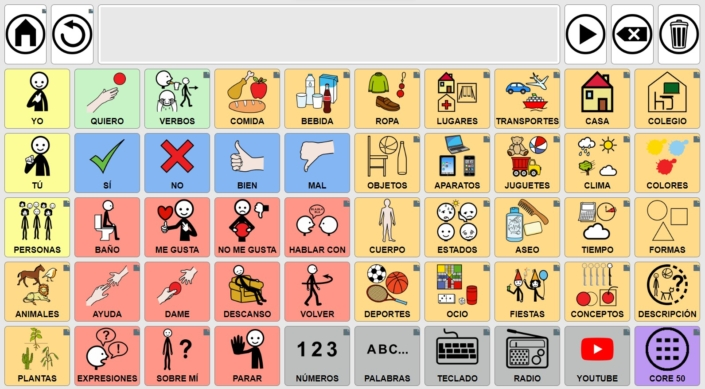
\includegraphics[scale = 0.8]{images/comunicador.jpg}
\centering
\caption{Comunicador AsTeRISCS Grid desarrollado por ARASAAC. Extraído de \cite{asterics_grid_comunicador}}
\label{fig:comunicador}
\end{figure}

Aunque los comunicadores electrónicos son herramientas verdaderamente útiles para mejorar la comunicación de las personas, presentan ciertas limitaciones. Una de las principales es la dificultad para formar frases complejas y gramaticalmente correctas, ya que, para facilitar y simplificar su uso, estos sistemas suelen incluir solamente palabras clave en su forma básica, sin distinguir número, género o tiempo verbal, cosa que restringe en gran medida la fluidez y expresividad de la comunicación.

Algunos de los comunicadores que existen actualmente en el mercado ya emplean diferentes métodos para abordar este problema, pero existe todavía un amplio margen de mejora. Las recientes innoviaciones en el campo de la inteligencia artificial y el procesamiento de lenguaje natural ofrecen nuevas oportunidades para superar estas limitaciones. En particular, los modelos de lenguaje grandes (LLMs) tienen un gran potencial para transformar el uso de estos sistemas, pudiendo proporcionar una generación de texto mucho más natural.

\section{Objetivos}

Los objetivos principales de este proyecto son los siguientes:
\begin{enumerate}
\item Investigar sobre los enfoques actuales para la generación de frases en el sector de los SAAC.
\item Adaptar y evaluar modelos de lenguaje grandes de acceso público que son utilizados actualmente para la generación de frases en herramientas SAAC.
\item Comparar los resultados que se obtienen con los LLMs respecto a otros comunicadores que permiten la generación de frases que se encuentran en el mercado.
\end{enumerate}

\section{Estructura de la memoria}

Este documento está dividido en 5 capítulos. El Capítulo \ref{cap1} proporciona la motivación y los objetivos del trabajo, estableciendo también el contexto de la investigación. El Capítulo \ref{cap2} presenta los conceptos esenciales, comenzando con una visión general del aprendizaje automático y seguido de una explicación detallada de las redes neuronales, tranformers y modelos de lenguaje grandes. En el Capítulo \ref{cap3} se detallan los modelos de lenguaje utilizados, los métodos para su ajuste y adaptación al contexto y las técnicas de evaluación. El Capítulo \ref{cap4} describe los datos utilizados, el entrenamiento de los modelos y los resultados obtenidos. Finalmente, el Capítulo \ref{cap5} ofrece un resumen de los resultados, evalúa los objetivos alcanzados y sugiere posibles direcciones para futuras investigaciones.

%\section{Notes bibliografiques} %%%%% Opcional

%????? ????????????? ????????????? ????????????? ????????????? ?????????????

%%%%%%%%%%%%%%%%%%%%%%%%%%%%%%%%%%%%%%%%%%%%%%%%%%%%%%%%%%%%%%%%%%%%%%%%%%%%%%%
%                         CAPITOLS (tants com calga)                          %
%%%%%%%%%%%%%%%%%%%%%%%%%%%%%%%%%%%%%%%%%%%%%%%%%%%%%%%%%%%%%%%%%%%%%%%%%%%%%%%

\chapter{Fundamentos}\label{cap2}

En este capítulo se abordan los conceptos fundamentales necesarios para comprender el funcionamiento de los modelos de lenguaje grandes. En primer lugar, se presenta una visión general del aprendizaje automático, seguido de una explicación detallada sobre las redes neuronales, con un efoque particular en su aplicación en el procesamiento de texto. A continuación, se explora la arquitectura de los transformers y se presentan los modelos de lenguaje grandes, explicando detalladamente su funcionamiento.

\section{Aprendizaje automático}

El aprendizaje automático (ML, por su nombre en inglés, \textit{machine learning}) es una disciplina dentro de la inteligencia artificial que se centra en el desarrollo y estudio de algoritmos y modelos que permiten que los sistemas puedan relizar tareas específicas sin haber sido explícitamente programados para ello. Este término fue acuñado por Arthur Samuel en el año 1959, quien creo uno de los primeros programas exitosos de esta disciplina, conocido como \textit{the Samuel Ckeckers-playing Program} \cite{samuelCheckers} (el programa de juego de damas de Samuel).

Tom Mitchell \cite{mitchell1997mcgraw} define el proceso de aprendizaje de los programas en el campo del \textit{machine learning} de la siguiente manera:

\begin{displayquote}
\textit{"Se dice que un programa aprende de la experiencia $E$ con respecto a alguna clase de tarea $T$, y medida de rendimiento $P$, si su rendimiento en tareas en $T$, medido por $P$, mejora con la experiencia $E$."}
\end{displayquote}

Aunque la idea principal del aprendizaje automático es esta, econtramos diferentes enfoques dependiendo del tipo de tarea que se quiera llevar a cabo, de la naturaleza de esta, de la medida del rendimiento que se utiliza para evaluar el sistema y del tipo de entrenamiento o experiencia que le proporcionamos a este.

Generalmente, los enfoques para el entrenamiento de algoritmos se agrupan en:

\begin{itemize}
	\item \textbf{Aprendizaje supervisado}, cuyo objetivo es, a partir de unos datos de entrenamiento, encontrar la función $f$ que realice el mejor mapeo posible entre un conjunto de entradas $X$ y sus salidas correspondientes $Y$, de manera que $(X, Y) = (X, f(X))$.
	\item \textbf{Aprendizaje no supervisado}, que trata de modelar la estructura subyacente de un conjunto de datos para identificar relaciones y patrones, permitiendo así un entendimiento más profundo de los mismos.
	\item \textbf{Aprendizaje semi-supervisado}, que cae entre el supervisado y el no supervisado y utiliza una porción de datos etiquetados y no etiquetados.
	\item \textbf{Aprendizaje por refuerzo}, donde el algoritmo aprende a través de retroalimentaciones que va recibiendo, ajustando sus acciones con el objetivo de maximizar una recompensa acumulada a lo largo del tiempo \cite{mirtaheri2022machine}.

\end{itemize}

La tarea principal de este trabajo se llevará a cabo utilizando técnicas de aprendizaje supervisado.

Otro concepto importante dentro del aprendizaje automático es el aprendizaje profundo (\textit{deep learning}). El aprendizaje profundo es subconjunto dentro del aprendizaje automático que emplea algoritmos basados en redes neuronales. Dentro de este encontramos métodos como las redes neuronales profundas, las redes neuronales recurrentes, las redes neuronales convolucionales y los transformers, entre otros. Estos métodos tienen aplicaciones significativas en una gran variedad de ámbitos, entre los que se encuentra el procesamiento de lenguaje natural, disciplina en la que se enmarca este trabajo. En las siguientes secciones explicaremos con detalle los conceptos de redes neuronales y transformers.

\section{Redes neuronales}
%https://web.stanford.edu/~jurafsky/slp3/ed3book_jan72023.pdf

El primer modelo de red neuronal artificial fue creado en 1943 por Warren McCulloch y Walter Pitts, y se conoce como \textit{McCulloch-Pitts neuron} \cite{mcculloch1943logical}. Este era un modelo simplificado que imitaba el comportamiento de una neurona natural. Esto dio inicio a un proceso de investigación de las redes neuronales desde dos enfoques distintos: uno centrado en los procesos biológicos del cerebro y otro en la aplicación de las redes neuronales para la inteligencia artificial. Las redes neuronales modernas, aunque inspiradas en estas primeras ideas, han evolucionado significativamente y ya no se basan directamente en las inspiraciones biológicas iniciales.

Las redes neuronales modernas están compuestas por pequeñas unidades de cómputo conocidas como neuronas o nodos, conectadas entre si a través de enlaces para permitir la transmisión de señales entre estas. Los nodos están organizados en capas, de manera que un nodo en una capa está conectado a todos los nodos de la capa siguiente. Existen tres tipos de capa: capa de entrada (\textit{input layer}), capas ocultas (\textit{hidden layers}) y capa de salida (\textit{output layer}). 

La arquitectura más simple de red neuronal es la de perceptrón. Este tipo de modelo surgió como método para tareas de clasificación binaria, en las que se debe decidir si un determinado \textit{input} pertenece o no a una clase, aunque se amplió para abarcar también tareas de clasificación multiclase. Es un tipo de clasificador lineal, por lo que hace sus predicciones basándose en una función de predicción lineal que combina un conjunto de pesos con el vector de entrada. Este tipo de arquitectura sirve como base para arquitecturas de redes neuronales mucho más complejas.

\begin{figure}[h]
	\centering
	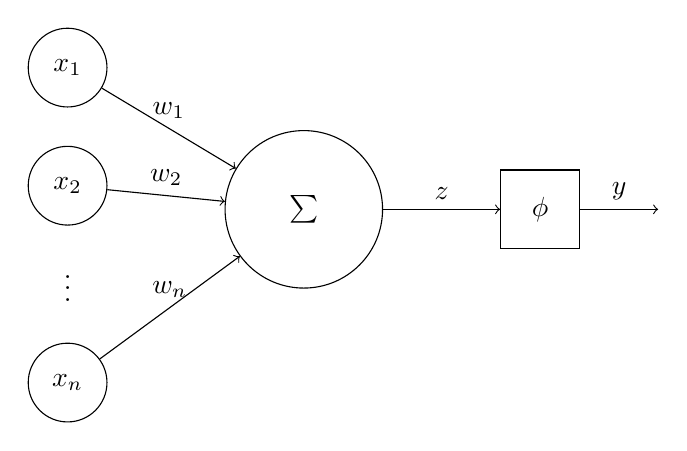
\begin{tikzpicture}
		\tikzstyle{roundnode} = [draw, shape = circle, minimum size = 1cm]
		\tikzstyle{activation} = [draw, shape = rectangle, minimum size = 1cm]
	% Nodos
		\node[roundnode](circle1) at (0, 3.5) {$x_1$};
		\node[roundnode](circle2) at (0, 2) {$x_2$};
		\node (dots) at (0, 0.8) {$\vdots$};
		\node[roundnode](circle3) at (0, -0.5) {$x_n$};

		\node[roundnode, minimum size = 2cm](sum) at (3, 1.7) {$\sum$};
		\node[activation] (act) at (6, 1.7) {$\phi$};

	% Enlaces
		\draw[->]  (circle1) -- (sum) node[midway, above] {$w_1$};
		\draw[->] (circle2) -- (sum) node[midway, above] {$w_2$};
		\draw[->] (circle3) -- (sum) node[midway, above] {$w_n$};
		\draw[->] (sum) -- (act) node[midway, above] {$z$};
		\draw[->] (act) -- (7.5, 1.7) node[midway, above] {$y$};


	\end{tikzpicture}
	\caption{Esquema de perceptrón simple}
	\label{fig:perceptronSimple}	
\end{figure}


Tal y como vemos en la Figura \ref{fig:perceptronSimple}, en la arquitectura de perceptrón simple encontramos solamente una neurona, que toma un vector $x$ como entrada. La neurona calcula la combinación lineal de los elementos del vector $x_1, x_2, ..., x_n$ con los pesos correspondientes $w_1, w_2, ..., w_n$, añadiendo al resultado un valor conocido como umbral o \textit{bias term}:

 \begin{equation}
\label{form:calcularZ}
z = b + \sum_{i = 1}^n w_i x_i
\end{equation}

 A este resultado se le aplica una función $\phi$ conocida como función de activación, y finalmente se devuelve un solo valor $y$ como salida:

\begin{equation}
y = \phi(z) = 
\begin{cases}
	1 & \text{si } z \ge 0 \\
	0 & \text{si } z < 0
\end{cases}
\end{equation}

El entrenamiento de las redes neuronales consiste en ajustar los distintos pesos de la red de manera que produzca las salidas más acertadas posibles. En el caso de las redes de perceptrón, al contar con solamente una neurona, este proceso resulta relativamente sencillo. El primer paso es inicializar el vector de pesos con valores aleatorios y calcular la salida de cada vector de entrada del conjunto de entrenamiento. A continuación, se comprueba si la predicción ha sido correcta. Si no lo ha sido, el vector de pesos se modifica utilizando la siguiente fórmula:

\begin{equation}
w = w - \lambda(\hat{y}-y)x
\end{equation}

donde $\lambda$ es la tasa de aprendizaje, $\hat{y}$ es el \textit{output} predicho por el modelo y $y$ es la clasificación real. Este proceso se puede realizar muestra a muestra (\textit{online}) o para un subconjunto de muestras de entrenamiento (\textit{batch}).

Así, estos pasos se repiten durante un número determinado de iteraciones o hasta que el modelo converge.

Este modelo de perceptrón tiene una limitación principal: el modelo solo converge si las dos clases en las cuales debe clasificar las muestras son linealmente separables. En caso de que no lo sean, los pesos oscilarán indefinidamente, hasta que el número máximo de iteraciones se alcance. Para solventar esta limitación existen modelos de redes neuronales mucho más complejos, con más neuronas y que utilizan funciones de activación no lineales. El modelo más conocido de este tipo es el de perceptrón multicapa (MLP, por su nombre en inglés: \textit{Multi-Layer Perceptron}).

\subsection{Perceptrón multicapa} \label{perceptronmulticapa}
El modelo de perceptrón multicapa es una evolución del modelo de perceptrón simple que tiene como objetivo el poder resolver problemas no lineales. La idea principal detrás de este modelo es la combinación de varios perceptrones simples en una única arquitectura más compleja. En esta arquitectura podemos encontrar un número elevado de neuronas, conectadas entre sí y organizadas en capas. Encontramos tres tipos de capas: una capa de entrada (\textit{input layer}), una o más capas ocultas (\textit{hidden layers}) y una capa de salida (\textit{output layer}) (ver Figura \ref{fig:perceptronMulticapa}).

\begin{figure}[h]
    \centering
    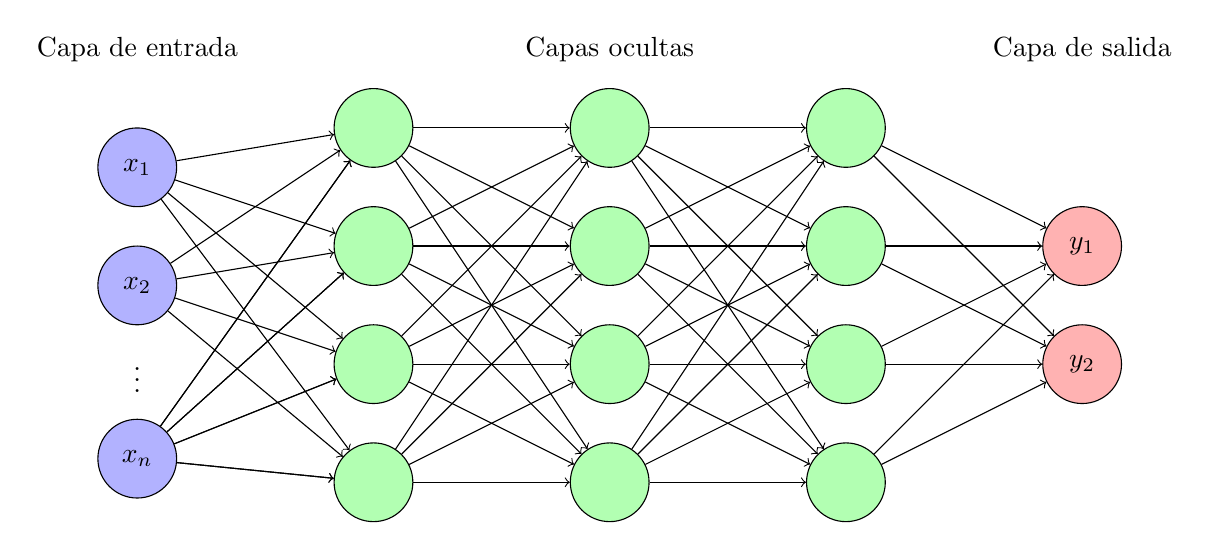
\begin{tikzpicture}
        \tikzstyle{input} = [draw, circle, fill=blue!30, minimum size=1cm]
        \tikzstyle{hidden} = [draw, circle, fill=green!30, minimum size=1cm]
        \tikzstyle{output} = [draw, circle, fill=red!30, minimum size=1cm]
        
        % Nodos de entrada
        \node[input](input1) at (0, 3.5) {$x_1$};
        \node[input](input2) at (0, 2) {$x_2$};
        \node (dots) at (0, 0.9) {$\vdots$};
        \node[input](input3) at (0, -0.2) {$x_n$};

        % Nodos ocultos 1
        \node[hidden](hidden1) at (3, 4) {};
        \node[hidden](hidden2) at (3, 2.5) {};
        \node[hidden](hidden3) at (3, 1) {};
        \node[hidden](hidden4) at (3, -0.5) {};

        % Nodos ocultos 2
        \node[hidden](hidden5) at (6, 4) {};
        \node[hidden](hidden6) at (6, 2.5) {};
        \node[hidden](hidden7) at (6, 1) {};
        \node[hidden](hidden8) at (6, -0.5) {};

        % Nodos ocultos 3
        \node[hidden](hidden9) at (9, 4) {};
        \node[hidden](hidden10) at (9, 2.5) {};
        \node[hidden](hidden11) at (9, 1) {};
        \node[hidden](hidden12) at (9, -0.5) {};

        % Nodos de salida
        \node[output](output1) at (12, 2.5) {$y_1$};
        \node[output](output2) at (12, 1) {$y_2$};

        % Enlaces desde la capa de entrada a la primera capa oculta
        \foreach \i in {1,2,3}
            \foreach \j in {1,2,3,4}
                \draw[->] (input\i) -- (hidden\j);

        \draw[->] (input3) -- (hidden1);
        \draw[->] (input3) -- (hidden2);
        \draw[->] (input3) -- (hidden3);
        \draw[->] (input3) -- (hidden4);
        
        % Enlaces desde la primera capa oculta a la segunda capa oculta
        \foreach \i in {1,2,3,4}
            \foreach \j in {5,6,7,8}
                \draw[->] (hidden\i) -- (hidden\j);

        % Enlaces desde la segunda capa oculta a la tercera capa oculta
        \foreach \i in {5,6,7,8}
            \foreach \j in {9,10,11,12}
                \draw[->] (hidden\i) -- (hidden\j);

        % Enlaces desde la tercera capa oculta a la capa de salida
        \foreach \i in {9,10,11,12}
            \foreach \j in {1,2}
               \draw[->] (hidden\i) -- (output\j);

        % Textos de las capas
        \node at (0, 5) {Capa de entrada};
        \node at (6, 5) {Capas ocultas};
        \node at (12, 5) {Capa de salida};
    \end{tikzpicture}
    \caption{Esquema de perceptrón multicapa}
    \label{fig:perceptronMulticapa}	
\end{figure}

Cada una de las neuronas de una capa está conectada a todas las neuronas de la capa siguiente, y cada uno de los enlaces tiene asociado un peso $w$. De manera similar al modelo de perceptrón simple, los datos se introducen en el modelo en forma de vector a través de la capa de entrada. El ajuste de pesos en el entrenamiento del modelo de perceptrón multicapa se realiza mediante el algoritmo de retropropagación (en inglés, \textit{backpropagation algorithm}) \cite{Rojas1996}. El algoritmo de retropropagación se puede desglosar en cuatro fases:

\begin{enumerate}
	\item \textbf{Computación hacia adelante (\textit{feed-forward})}: se realiza una pasada hacia adelante a través de la red, desde la capa de entrada hasta la capa de salida. En esta fase, se calculan las salidas de las neuronas utilizando la Ecuación \ref{form:calcularZ} y aplicando sobre este resultado una función de activación no lineal, por ejemplo la función sigmoide, la tangente hiperbólica (\textit{tanh}) o la rectificada lineal (\textit{ReLU}). El uso de este tipo de funciones permite que el modelo pueda aplicarse a problemas no lineales. Al llegar a a la capa de salida, se calcula la predicción final del modelo.
	\item \textbf{Retropropagación en la capa de salida}: a continuación, se calcula el error en la capa de salida comparando las predicciones del modelo con los valores reales. Posteriormente, se calculan los gradientes del error respecto a los pesos de esta capa.
	\item \textbf{Retropropagación en las capas ocultas}: utilizando los gradientes obtenidos en la capa de salida, el error se propaga hacia atrás a través de las capas ocultas, ajustando los gradientes del error respecto a los pesos en cada una de estas.
	\item \textbf{Actualización de los pesos}: finalmente, se actualizan los pesos de la red utilizando los gradientes calculados en las fases anteriores mediante el método de descenso de gradiente u otro algoritmo de optimización similar.
\end{enumerate}

Este proceso se repite de manera iterativa hasta alcanzar el número máximo de iteracoines o hasta que el modelo converge.

\subsection{Redes neuronales para secuencias de texto}

% Probabilistic neural networks (book1)

El procesamiento de secuencias de texto utilizando redes neuronales es una técnica fundamental en el campo del procesamiento de lenguaje natural. Dado que las redes neuronales operan utilizando vectores numéricos, es necesario transformar las secuencias de texto en vectores antes de poder procesarlas. Este proceso se realiza en varias etapas, que se detallan a continuación:

\begin{enumerate}
	\item \textbf{Tokenización y conversión a índices}: el primer paso consiste en convertir la frase en una secuencia de palabras o tokens. Una vez obtenida la lista de tokens, se asigna a cada uno un número que servirá como índice.
	\item \textbf{Transformación de palabras en vectores}: los índices numéricos se transforman en vectores utilizando \textit{embeddings}. Los \textit{embeddings} son representaciones vectoriales densas que capturan las características semánticas de las palabras.
	\item \textbf{Creación de la matriz de \textit{embeddings}}: una vez que se han obtenido los vectores asociados a cada una de las palabras, se puede construir una matriz de \textit{embeddings} que representa la frase completa. Esta matriz facilita la entrada secuencial de los vectores en la red neuronal.
\end{enumerate}

Cada palabra en la secuencia de texto es procesada por la red neuronal de manera secuencial. En la siguiente sección se presentan las redes neuronales recurrentes (RNNs), un tipo de red neuronal que es ampliamente utlizado para el procesamiento de secuencias de texto.

\subsubsection{Redes neuronales recurrentes (RNN)} \label{rnn}
Las redes neuronales recurrentes (en inglés, \textit{recurrent neural networks} (RNN)) son un tipo de red neuronal que mapean desde un conjunto de entrada a otro de salida de manera que la predicción $y_t$ depende no solo de la de entrada $x_t$ sino también del estado oculto del sistema, $h_t$ \cite{murphy2022probabilistic}. El estado oculto $h_t$ es una representación interna de la red en el momento de tiempo $t$ que captura información relevante que ha sido procesada anteriormente. Se actualiza con el tiempo a medida que se procesan los datos. Este tipo de modelos se pueden utilizar para la generación, clasificación y traducción de texto.

El proceso que siguen este tipo de redes es el siguiente. En primer lugar, se inicializa la red con un estado oculto $h_0$, que puede ser un vector de ceros o una inicialización aprendida. Para cada elemento en la secuencia de entrada, la red actualiza su estado oculto y produce una salida. Así, en el momento de tiempo t, la entrada $x_t$ y el estado oculto previo $h_{t-1}$ se combinan para generar el nuevo estado oculto $h_t$. Este se calcula utilizando la fórmula:

\begin{equation}
h_t = f(W_hh_{t-1} + W_xx_t + b_h)
\end{equation}

donde $W_h$ y $W_x$ son las matrices de pesos asociadas al estado oculto y a las entradas respectivamente, $f$ es una función no lineal y $b_h$ es un vector de sesgos. La salida $y_t$ se obtiene a partir del estado oculto $h_t$:

\begin{equation}
y_t = g(W_yh_t + b_y)
\end{equation}

donde $W_y$ es una matriz de pesos, $g$ es la función de activación y $b_y$ es un vector de sesgos \cite{sutskever2014sequencesequencelearningneural}.

El proceso se repite para cada elemento de la secuencia de entrada, propagando así la información relevante anterior a través de los estados ocultos.

Uno de los principales problemas de las RNN es la dificultad para recordar información a largo plazo, pues se ha comprobado que, si el modelo es entrenado con secuencias de entrada largas, la importancia de las primeras palabras que son procesadas tiende a ir perdiendose a medida que se procesa el resto de la secuencia. Esto limita la capacidad de este tipo de redes para capturar dependencias a largo plazo en secuencias largas.

%\subsubsection{Redes neuronales convolucionales (CNN)}
%El funcionamiento de las redes neuronales convolucionales (\textit{convolutional neural networks (CNN)} se basa en el calculo de una función de un vecindario local para cada una de las entradas utilizando pesos compartidos. Son una buena alternativa a las redes neuronales recurrentes, pues son sustancialmente más sencillas de entrenar, ya que no necesitan mantener el estado oculto a largo plazo. Se pueden utilizar en tareas de clasificación y de generación de texto.

\subsection{Arquitectura \textit{encoder-decoder}} \label{encdec}

Los modelos \textit{encoder-decoder}, también conocidos como modelos \textit{seq2seq} (\textit{sequence-to-sequence}) son modelos capaces de generar secuencias de salida contextualmente apropiadas y de longitud arbitraria a partir de una secuencia de entrada. Estos modelos pueden generar secuencias de salida de longitud variable a partir de secuencias de entrada también de longitud variable, es decir, secuencias con longitudes distintas en la entrada y la salida.
Son modelos ampliamente utilizados en tareas como el resumen de textos, la respuesta a preguntas, el diálogo y la traducción automática \cite{jurafsky2023speech}.

Este tipo de modelos están formados por dos componentes principales: el \textit{encoder} (en español, codificador) y el \textit{decoder} (decodificador). El \textit{encoder} es la primera parte del modelo. Se encarga de mapear las secuencias de entrada a una representación intermedia contextualizada $h$ en forma de vector. Este vector $h$ captura la información relevante de cada elemento de la secuencia de entrada y sus contextos. A continuación, el \textit{decoder} toma el vector de contexto $h$ y, a partir de este, genera la secuencia de salida. Además, el \textit{decoder} puede tener en cuenta también los estados del \textit{encoder} gracias al mecanismo de atención, que se explicará en detalle en la sección \ref{atencion} \cite{sriram2017coldfusiontrainingseq2seq}.

Esta arquitectura se puede implementar utilizando diversos tipos de redes neuronales, incluyendo los transformers, como veremos en la sección \ref{transformers}, o las redes neuronales recurrentes.

\subsection{Atención} \label{atencion}

Tal y como se ha explicado en las secciones anteriores, en las redes neuronales clásicas, el cálculo de cada capa se realiza mediante una combinación lineal de los vectores de entrada y los correspondientes pesos, seguida de la aplicación de una función de activación. Esta operación se representa matemáticamente como $Z = \phi(XW)$, donde $X$ es el vector de entrada, $W$ es el vector de pesos, $\phi$ es la función de activación y $Z$ son las salidas producidas en las capas \cite{murphy2022probabilistic}. 

Sin embargo, los modelos de redes neuronales pueden volverse aún más flexibles y potentes si permitimos que los pesos dependan de los \textit{inputs}. Esta interacción multiplicativa, donde los pesos son dinámicos y dependen de las entradas, se conoce como mecanismo de atención. Formalmente, puede expresarse como $Z = \phi(XW(X))$.

De manera más general, el mecanismo de atención puede describirse mediante la fórmula $Z = \phi(VW(Q, K))$. En este contexto:

\begin{itemize}
\item $Q$ (\textit{queries}) es un conjunto derivado de $X$ que describe qué es lo que busca cada palabra, es decir, con qué otro tipo de palabras puede estar relacionada.
\item $K$ (\textit{keys}) es otro conjunto derivado de $X$ que se usa para describir cuáles son las propiedades de las palabras.
\item $V$ (\textit{values}) es un conjunto también derivado de $X$ que describe cómo cada entrada debe ser transmitida hasta la salida.
\end{itemize}

Los vectores de \textit{queries}, \textit{keys} y valores se obtienen procesando las palabras mediante tres redes neuronales independientes.

Cuando se utiliza la atención para calcular una salida $z_i$, se utiliza la \textit{query} $q_i$ correspondiente  y se compara con cada una de las claves $k_j$ de todas las otras palabras de la secuencia, calculando cuál es su nivel de relación con cada una. Esto se realiza mediante el producto escalar entre el vector \textit{query} y los vectores \textit{key} de las otras palabras de la secuencia, de la siguiente manera:

\begin{equation}
\alpha_{ij} = softmax(q_i \cdot k_j)
\end{equation}

Se utiliza la función \textit{softmax} para normalizar los resultados y poder así crear el correspondiente vector de pesos. Así, el resultado se representa como $\alpha_{ij}$ y debe cumplir las siguientes condiciones:

\begin{equation}
0 \le \alpha_{ij} \le 1
\end{equation}

\begin{equation}
\sum_j\alpha_{ij} = 1
\end{equation}

El coeficiente $\alpha_{ij}$ determina cuánto peso se debe dar a cada valor $v_j$ en la combinación final, y representa el nivel de importancia que tiene cada palabra de la secuencia sobre la palabra $i$. La salida $z_i$ se calcula entonces como una suma ponderada de los valores $v_j$, donde los pesos son los coeficientes calculados:

\begin{equation}
z_i = \sum_j\alpha_{ij}v_j
\end{equation}

Este enfoque permite que los \textit{outputs} del modelo sean una combinación dinámica ponderada de los \textit{inputs}, lo que hace que este tipo de sistemas sean mucho más efectivos para una amplia gama de tareas, como la traducción automática, el resumen de textos o la generación de texto entre otros. \cite{murphy2022probabilistic, jurafsky2023speech}

\section{Transformers} \label{transformers}

En esta sección presentaremos la arquitectura de transformers. Los modelos basados en transformers emplean una arquitectura \textit{encoder-decoder} que utiliza el mecanismo de atención, descrito en la sección anterior. La arquitectura de los transformers fue introducida en el artículo "\textit{Attention is All You Need"} \cite{vaswani2023attentionneed}, publicado en 2017. Esta supuso una gran revolución en diversas áreas del aprendizaje automático por su capacidad para manejar de manera efectiva secuencias largas y complejas \cite{dai2019transformerxlattentivelanguagemodels}. Actualmente, hay una gran cantidad de modelos basados en esta arquitectura que se utilizan en el área del procesamiento de lenguaje natural.

\subsection{Estructura del Transformer}

Tal y como se ha mencionado anteriormente, la arquitectura de transformers utiliza el modelo \textit{encoder-decoder} introducido en la sección \ref{encdec}. En este caso, se utilizan un total de seis bloques de \textit{encoder} y seis de \textit{decoder}, cada uno de los cuales contiene varias capas y mecanismos que facilitan el procesamiento eficiente de las secuencias de datos.

En general, los transformers utilizan tres tipos de capas: capas lineales simples, capas de \textit{multi-head attention} y capas donde encontramos redes neuronales de tipo \textit{feed forward}. En la figura \ref{fig:transformers} encontramos el esquema de la estructura de los \textit{encoders} y  \textit{decoders}. Tal y como se puede observar, el \textit{encoder} está formado por una primera capa de \textit{multi-head attention} y, a continuación, una red neuronal de tipo \textit{feedforward} completamente conectada, además de las capas de normalización que encontramos después de estas. Por lo que respecta al \textit{decoder}, lo conforman dos capas de autoatención y una red neuronal, también con capas de normalización después de estas. \cite{jurafsky2023speech, multiheaddotproduct}

\begin{figure}[h]
    \centering
    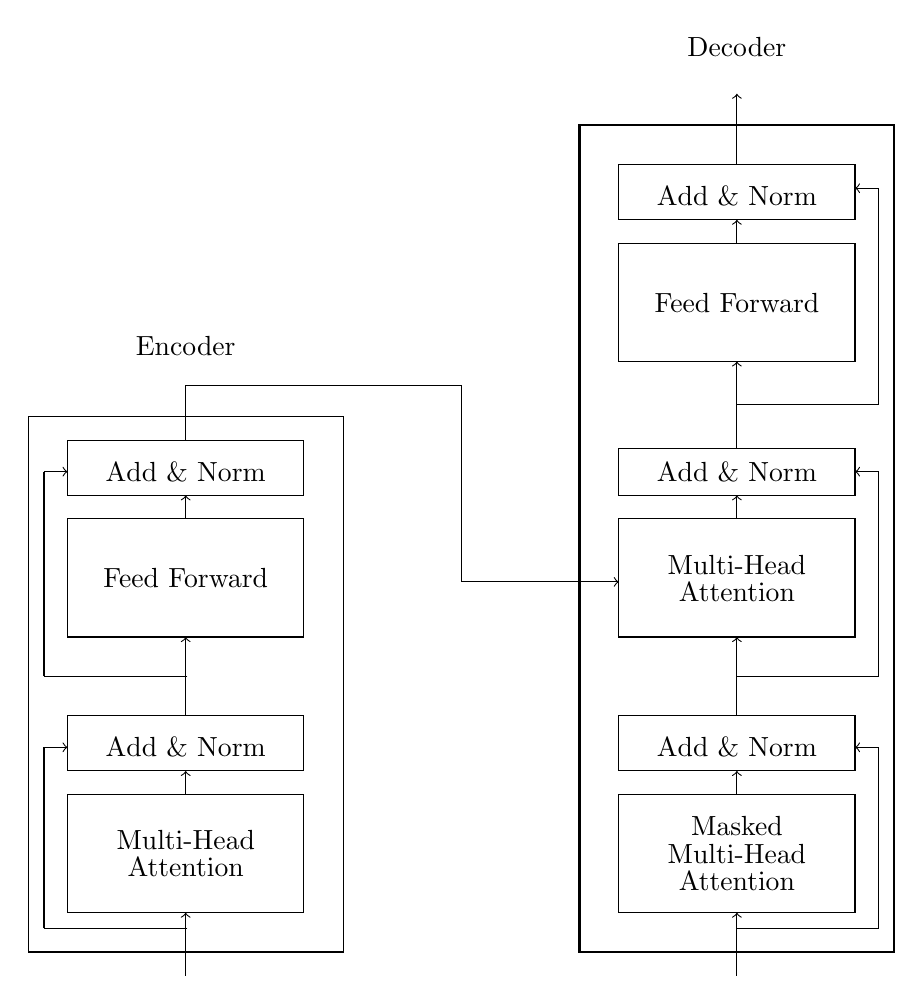
\begin{tikzpicture}[scale=1, transform shape]

        % Encoder
        \draw (0,0) rectangle (4,6.8);
        \node at (2,7.7) {Encoder};
        
        % Encoder components
        \draw (0.5,0.5) rectangle (3.5,2);
        \node at (2,1.25) {\shortstack{Multi-Head\\Attention}};
        
        \draw (0.5,2.3) rectangle (3.5,3);
        \node at (2,2.6) {Add \& Norm};
        
        \draw (0.5,4) rectangle (3.5,5.5);
        \node at (2,4.75) {Feed Forward};
        
        \draw (0.5,5.8) rectangle (3.5,6.5);
        \node at (2,6.1) {Add \& Norm};
        
        % Decoder
        \draw[thick] (7,0) rectangle (11,10.5);
        \node at (9,11.5) {Decoder};
        
        % Decoder components
        \draw (7.5,0.5) rectangle (10.5,2);
        \node at (9,1.25) {\shortstack{Masked\\Multi-Head\\Attention}};
        
        \draw (7.5,2.3) rectangle (10.5,3);
        \node at (9,2.6) {Add \& Norm};
        
        \draw (7.5,4) rectangle (10.5,5.5);
        \node at (9,4.75) {\shortstack{Multi-Head\\Attention}};
        
        \draw (7.5,5.8) rectangle (10.5,6.4);
        \node at (9,6.1) {Add \& Norm};
        
        \draw (7.5,7.5) rectangle (10.5,9);
        \node at (9,8.25) {Feed Forward};
        
        \draw (7.5,9.3) rectangle (10.5,10);
        \node at (9,9.6) {Add \& Norm};
        
        % Encoder lines
	\draw[->] (2, -0.3) -- (2, 0.5);
	\draw[->] (2, 2) -- (2, 2.3);
	\draw[->] (2, 3) -- (2, 4);
	\draw[->] (2, 5.5) -- (2, 5.8);
	\draw (2.02, 0.3) -- (0.2, 0.3);
	\draw (0.2, 0.3) -- (0.2, 2.6);
	\draw[->] (0.2, 2.6) -- (0.5, 2.6);

	\draw (2.02, 3.5) -- (0.2, 3.5);
	\draw (0.2, 3.5) -- (0.2, 6.1);
	\draw[->] (0.2, 6.1) -- (0.5, 6.1);

	% Decoder lines
	\draw[->] (9, -0.3) -- (9, 0.5);
	\draw[->] (9, 2) -- (9, 2.3);
	\draw[->] (9, 3) -- (9, 4);
	\draw[->] (9, 5.5) -- (9, 5.8);
	\draw[->] (9, 6.4) -- (9, 7.5);
	\draw[->] (9, 9) -- (9, 9.3);
	\draw[->] (9, 10) -- (9, 10.9);

	\draw (9, 0.3) -- (10.8, 0.3);
	\draw (10.8, 0.3) -- (10.8, 2.6);
	\draw[->] (10.8, 2.6) -- (10.5, 2.6);

	\draw (9, 3.5) -- (10.8, 3.5);
	\draw (10.8, 3.5) -- (10.8, 6.1);
	\draw[->] (10.8, 6.1) -- (10.5, 6.1); 

	\draw (9, 6.95) -- (10.8, 6.95);
	\draw (10.8, 6.95) -- (10.8, 9.7);
	\draw[->] (10.8, 9.7) -- (10.5, 9.7);


	\draw (2, 6.5) -- (2, 7.2);
	\draw (2, 7.2) -- (5.5, 7.2);
	\draw (5.5, 7.2) -- (5.5, 4.7);
	\draw[->] (5.5, 4.7) -- (7.5, 4.7);

        
    \end{tikzpicture}
    \caption{Esquema de la arquitectura de los transformers}
    \label{fig:transformers}
\end{figure}

La idea principal del transformer es, a lo largo de esta serie de capas, poder construir representaciones contextualizadas cada vez más acertadas de los significados de las palabras o \textit{tokens} de las secuencias de entrada. Así, en las distintas capas del transformer, para obtener la representación de una palabra, se combina la información de la representación obtenida en la capa anterior con la información de las representaciones de las palabras vecinas. El objetivo es producir la versión contextualizada de cada palabra, representando lo que significa esta en el contexto particular en que se encuentra. \cite{jurafsky2023speech}

A continuación se explica con más detalle los procesos que ocurren dentro de cada capa.

\subsection{Capas de \textit{multi-head attention}}
Las capas de \textit{multi-head attention} suponen la verdadera innovación de la arquitectura de transformers \cite{jurafsky2023speech}, pues es en estas donde el modelo aplica el mecanismo de atención.  En el caso de los transformers, se utiliza una variación del mecanismo de atención explicado en la sección \ref{atencion}. Esta variación se conoce como \textit{scaled dot-product attention}. Igual que en el mecanismo general de atención, se utilizan tres matrices: la matriz de \textit{queries} $Q$, la de claves $K$ (por su nombre en inglés, \textit{keys}) y la de valores $V$ (\textit{values}). En este caso, el valor de atención se calcula utilizando la siguiente fórmula:

\begin{equation}
A(Q, K, V) = softmax(\frac{QK^t}{\sqrt{d_k}})
\end{equation}

donde $d_k$ es la dimensión del estado oculto de la fuente.

Como vemos, el cambio respecto al cálculo de atención descrito en la sección \ref{atencion} reside en que en este caso se añade el factor $\frac{1}{\sqrt{d_k}}$, que se utiliza para escalar el resultado obtenido, y conseguir así que las gradientes sean más estables, ya que si la secuencia de entrada fuera muy larga, la función \textit{softmax} puede devolver gradientes extremadamente pequeños, cosa que podria dificultar al modelo realizar un aprendizaje eficiente. \cite{multiheaddotproduct}

Aunque esta forma de cálculo de la atención es empleada por los transformers, estos no se quedan solamente en este concepto, sino que van un paso más allá y utilizan un tipo de atención algo más complejo conocido como \textit{multi-head attention}. Este proceso consiste en calcular distintas atenciones sobre las mismas \textit{queries} y pares clave-valor. Se utiliza este tipo de atención ya que las distintas palabras dentro de la secuencia de texto pueden estar relacionadas entre sí de muchas maneras distintas de manera simultánea. Capturar todas estas relaciones entre palabras es muy complicado si se utiliza un solo valor de atención.

Así, en las capas de \textit{multi-head attention} encontramos distintas capas de atención conocidas como \textit{heads} (cabezas), que calculan valores de atención de manera paralela. Cada una de estas tiene un conjunto distinto de parámetros que se aprende durante el entrenamiento, con los cuales hará el cálculo de atención entre las palabras de entrada. Utilizando parámetros distintos en cada cabeza se consigue que cada una se centre en aspectos distintos de las relaciones entre las palabras. El cálculo de atención para una cabeza $i$ se realiza mediante la siguiente fórmula:

\begin{equation}
H_i = A(QW_i^Q, KW_i^K, VW_i^V)
\end{equation}

Donde $W_i^Q$, $W_i^K$ y $W_i^V$ son las matrices de parámtetros asociadas a la \textit{query}, clave y valor respectivamente de la cabeza $i$. El valor de \textit{multi-head attention} se obtiene mediante la concatenación de los resultados de las cabezas. Para un total de $h$ cabezas de atención:

\begin{equation}
MultiHead(Q, K, V) = (H_1 \oplus H_2 \oplus ... \oplus H_h)W_O
\end{equation}

La matriz de parámetros $W_O$ proyecta la concatenación de los resultados de las $h$ cabezas de vuelta al subespacio original. \cite{cordonnier2021multiheadattentioncollaborateinstead, multiheaddotproduct, jurafsky2023speech}

\subsection{Capas de redes \textit{Feed Forward}}

Las capas \textit{feed forward} en la arquitectura de transformers están compuestas por redes neuronales independientes de tipo \textit{feed forward} (en español, redes de propagación hacia adelante). Este tipo de red neuronal es equivalente al modelo de perceptrón multicapa descrito en la Sección  \ref{perceptronmulticapa}.

Así, una red neuronal de tipo \textit{feed forward} es una red multicapa en la que, a diferencia de las redes neuronales recurrentes (RNN) explicadas en la sección \ref{rnn}, las conexiones entre neuronas no pueden formar ciclos. Esto implica que las señales siempre se propagan en una única dirección: desde la capa de entrada, a través de las capas ocultas, hacia la capa de salida. En la arquitectura de transformers, estas redes están completamente conectadas, lo que significa que las neuronas de una capa reciben las salidas de todas las neuronas de la capa anterior y envían sus salidas a todas las neuronas de la capa siguiente. Además, típicamente contienen solamente una capa oculta.

En los transformers, estas capas complementan las salidas de la capa de atención. Mientras que la capa de atención procesa cada palabra de la secuencia relacionandola con las demás palabras, las capas \textit{feed forward} procesan cada palabra de manera independiente. Este procesamiento independiente es crucial para mejorar la representación de las características extraídas de la capa de atención.

\subsection{Capas de normalización}

Las capas de normalización se encuentran detrás de tanto las capas de atención como las de redes \textit{forward}. En ellas se aplica el proceso de normalización de capas (en inglés, \textit{layer normalization} o \textit{layer norm} \cite{ba2016layernormalization}). Este tipo de normalización se utiliza para mejorar el rendimiento del entrenamiento de redes neuronales profundas, manteniendo los valores de la capa oculta dentro de un rango que facilita el entrenamiento basado en gradientes.

El proceso de normalización de capas toma como entrada un vector para cada palabra de la secuencia, y devuelve este mismo vector normalizado. El primer paso en el proceso es calcular la media $\mu$ y la desviación típica $\sigma$ del vector, de la siguiente manera:

\begin{equation}
\mu^l = \frac{1}{H} \sum_{i = 1}^Hx_i^l
\end{equation}

\begin{equation}
\sigma^l = \sqrt{\frac{1}{H} \sum_{i = 1}^H (x_i^l - \mu^l)^2}
\end{equation}

Donde $H$ es el número de unidades ocultas en la capa. A continuación, los componentes del vector se normalizan restando la media y desviación típica calculadas \cite{jurafsky2023speech}:

\begin{equation}
\hat{x} = \frac{(x - \mu)}{\sigma}
\end{equation}

Finalmente, se introducen parámetros de \textit{bias} $b$ y \textit{gain} $g$:

\begin{equation}
z = g\hat{x} + b
\end{equation}

%\section{Procesamiento del lenguaje natural} \label{nlp}

%El procesamiento de lenguaje natural (NLP, por su nombre en inglés \textit{Natural Language Processing}) es una rama de la inteligencia artificial que se ocupa del desarrollo de algoritmos y modelos para la realización de tareas relacionadas con el lenguaje humano. Más específicamente, involucra tareas como el modelado de lenguaje, clasificación de textos, recuperación y extracción de información, resumen de textos o traducción automática entre otras. \cite{alma997066713303706} 


\section{Modelos de lenguaje grandes} \label{modelosLenguajeGrandes}

Los modelos de lenguaje grandes (en inglés, \textit{Large Language Models} o LLM) representan una de las innovaciones más significativas en el campo del procesamiento de lenguaje natural. Estos modelos están basados en redes neuronales profundas, y generalmente utilizan la arquitectura de transformers. Estos modelos cuentan con miles de millones de parámetros, y pueden ser entrenados con enormes cantidades de texto, lo que hace que sean capaces de procesar y generar lenguaje humano con una gran fluidez, naturalidad y corrección.

Las tareas sobre las que se aplican son casos de generación condicional, es decir, generación de texto condicionado a un fragmento de entrada, conocido como \textit{prompt}. Los LLMs son modelos que están diseñados fundamentalmente para predecir la siguiente palabra de una secuencia de palabras \cite{jurafsky2023speech}. Aunque el ámbito de tareas sobre el que se pueden aplicar los LLMs pueda parecer reducido, la realidad es que la gran mayoría de tareas en el ámbito de NLP pueden ser enfocadas desde un punto de vista de generación condicional.

En la siguiente sección se explica cómo se deben introducir los datos de entrada al modelo mediante \textit{prompting}.

\subsection{\textit{Prompting}}

\textit{Prompting} se refiere al proceso mediante el cual se introducen una secuencia de entrada o \textit{query} al modelo a partir de la cual debe comenzar la tarea de generación de texto. Existen diversas maneras de crear estas \textit{prompts}. Las más utilizadas son las siguientes:

\begin{itemize}
	\item \textbf{\textit{Zero-shot prompting}}:
	\item \textbf{\textit{In-context learning }(ICL)}:
	\item \textbf{\textit{Chain-of-thought} (CoT)}:
	\item \textbf{\textit{Self consistency}}:
	\item \textbf{\textit{Tree of thought} (ToT)}:
\end{itemize}

Por ejemplo, para la tarea de responder preguntas, podriamos plantearlo de la siguiente manera:

En primer lugar, se proporciona al modelo una \textit{prompt} con la pregunta a contestar, con un formato que sugiera que después de la pregunta se espera una respuesta, por ejemplo: 

\begin{displayquote}
\centerline{"Pregunta: ¿Cuál es la capital de Francia? Respuesta: "}
\end{displayquote}

A continuación, el modelo calcula la probabilidad para cada palabra $w$ dentro de su vocabulario de que esta sea la palabra que continua la \textit{prompt}:

\begin{displayquote}
\centerline{$P(w|\text{Pregunta: ¿Cuál es la capital de Francia? Respuesta: })$}
\end{displayquote}

Los vocabularios en los LLMs se refieren al conjunto de palabras sobre las que trabajan. Así, habiendo calculado las probabilidades para todas las posibles palabras, encontraremos algunas con probabilidades más altas, entre las cuales debería encontrarse la palabra \textit{París}, que es la respuesta a la pregunta. El modelo deberia seleccionar esta palabra y, si se quiere generar una respuesta más larga, se calcula la siguiente probabilidad:

\begin{displayquote}
\centerline{$P(w|\text{Pregunta: ¿Cuál es la capital de Francia? Respuesta: París})$}
\end{displayquote}

El proceso puede seguir hasta que lleguemos al número de palabras deseadas.

Inicialmente, este cálculo de probabilidades se realizaba de manera secuencial, basando las predicciones en las distribuciones de probabilidad de las palabras dentro de un texto. Actualmente se utiliza la arquitectura de transformers, que permite procesar grandes cantidades de texto de manera eficiente y proporciona predicciones mucho más acertadas, pues tiene en cuenta el contexto en el que se encuentran las palabras y las relaciones entre estas \cite{burtsev2023working}.

Existen distintos enfoques para la selección de cuál es la palabra que sigue en la secuencia. Uno de los métodos más simples es utilizar el algoritmo de \textit{greedy decoding} \cite{gu2017trainablegreedydecodingneural}. El algoritmo \textit{greedy decoding} consiste en elegir la palabra con la probabilidad condicional más alta hasta el momento en cada instante.

\begin{equation}
\hat{w}_i = argmax_{w \in V} P(w | \{w_1, w_2, ..., w_{i-1}\})
\end{equation}

Con el tiempo se ha descubierto que este método llega a resultados subóptimos, pues al elegir siempre la palabra que es más probable que ocurra, tiende a generar textos excesivamente genéricos y repetitivos.

Existe una extension de este algoritmo conocida como \textit{beam search}, la cual ha demostrado ser más efectiva, sobretodo en tareas de traducción automática. La diferencia entre el algoritmo \textit{greedy decoding} y este, es que el \textit{beam search}, en lugar de quedarse solamente con la palabra con mayor probabilidad y crear una única respuesta, el algoritmo guarda $K > 1$ posibles respuestas (hipótesis) durante la decodificación. Así, en cada iteración, el algoritmo elige las K hipótesis con mayor \textit{score}:

\begin{equation}
p(w_1, w_2, ..., w_N) = \prod_{i = 1}^{N} p(w_i \mid w_1, w_2, ..., w_{i-1})
\end{equation}

Cuando estas se terminan de generar, selecciona la hipótesis con mayor probabilidad.

Aunque el rendimiento de \textit{beam search} es superior al \textit{greedy decoding}, en los LLM se suelen utilizar métodos más complejos, que proporcionan resultados más sofisticados. Estos métodos se conocen como métodos de generación por \textit{sampling}. Se explicarán con detalle en la siguiente sección.

\subsection{Métodos de generación por \textit{sampling}}

En términos generales, el proceso de \textit{sampling} consiste en seleccionar de manera aleatoria una serie de individuos de una muestra, teniendo (o no) en cuenta sus distribuciones de probabilidad. En el contexto de los LLM, esto se traduce en elegir las palabras que se generan en la secuencia de acuerdo con su probabilidad dentro del contexto definido por el modelo. De esta manera, es más probable seleccionar palabras con probabilidades altas y menos probable (aunque no imposible) elegir aquellas con probabilidades bajas.

 El algoritmo de generación por \textit{sampling} más sencillo se conoce como \textit{random sampling}, el cual consiste en seleccionar la siguiente palabra de la secuencia de manera aleatoria según la distribución de probabilidades proporcionada por el transformer. Sin embargo, este enfoque es demasiado simplista para la generación de texto de calidad, ya que al seleccionar las palabras de manera aleatoria, incluso las palabras poco comunes, que tendrán probabilidades bajas, pueden ser elegidas, lo que podría resultar en la generación de frases incorrectas o extrañas \cite{jurafsky2023speech}.

Debido a estas limitaciones, en los LLM se suelen emplear algoritmos más sofisticados, los cuales analizaremos en las siguientes secciones.

\subsubsection{\textit{Top-k sampling}}

El algoritmo de \textit{top-k sampling} es una generalización del \textit{greedy decoding} que consiste en seleccionar las $K$ palabras con mayor probabilidad de la distribución y aplicar \textit{random sampling} únicamente sobre este conjunto. Una vez se seleccionan las $K$ palabras del conjunto, sus probabilidades deben ser normalizadas según el nuevo conjunto. Las probabilidades normalizadas se calculan de la siguiente manera:

\begin{equation}
\hat{p}_i = \frac{p_i * \mathbb{1}\{i \leq K\}}{\sum_{j = 1}^K p_j}
\end{equation}

Donde $\mathbb{1}$ es la función característica, que indica si una palabra está dentro o no del conjunto de las $K$ más probables \cite{nadeem2020systematiccharacterizationsamplingalgorithms}.

\subsubsection{\textit{Nucleus sampling}}

El algoritmo de \textit{nucleus sampling} \cite{holtzman2020curiouscaseneuraltext}, también conocido como \textit{top-p sampling} también sigue la idea de eliminar de la distribución las palabras menos probables. Sin embargo, en lugar de seleccionar un número fijo de palabras, lo que hace es mantener el porcentaje $p$ más importante de la muestra. Así, dada una distribución $P(x |x_{1:i-1})$, las \textit{top-p} palabras del vocabulario $V^{(p)} \subset V$ se definen como el conjunto más pequeño que cumpla:

\begin{equation}
\sum_{x \in V^{(p)}} P(x | x_{1:i-1}) \ge p
\end{equation}

Al medir la probabilidad acumulada en lugar de un número fijo de palabras, se espera que esta medida sea más robusta incluso en contextos diversos, que podrían tener resultados muy distintos si se usara un número fijo de palabras. De nuevo, tras seleccionar el subconjunto de palabras del vocabulario se deben normalizar sus probabilidades.

Las probabilidades normalizadas de cada palabra en el vocabulario se pueden calcular como:

\begin{equation}
\hat{p}_i = \frac{p'_i}{\sum_{j = 1}^{|V|} p'_j}
\end{equation}

Donde $p'_i = p_i * \mathbb{1}\{\sum_{j = 1}^{i-1}p_j < P\}$ \cite{nadeem2020systematiccharacterizationsamplingalgorithms}.

\subsubsection{\textit{Tempered sampling}}

En el algoritmo de \textit{tempered sampling} \cite{nadeem2020systematiccharacterizationsamplingalgorithms} no crea un subconjunto de palabras del vocabulario, sino que ajusta la distribución de probabilidad de las palabras mediante una transformación. Para ello, se utiliza un parámetro $\tau$, que cumple $0 < \tau < 1$, según la siguiente fórmula:

\begin{equation}
\hat{p}_i = \frac{exp(log(p_i)/\tau)}{\sum_{j = 1}^{|V|}exp(log(p_j)/\tau)}
\end{equation}

Además, existe una variación de este algoritmo que se conoce como \textit{tempered top-k sampling}, el cual combina las transformaciones definidas por el algoritmo \textit{tempered sampling} y el \textit{top-k}. Así, la probabilidad normalizada se calcula:

\begin{equation}
\hat{p}_i = \frac{p'_i}{\sum_{j = 1}{|V|}p'_j}
\end{equation}

donde $p'_i = exp(log(p_i)/\tau * \mathbb{1}\{i \leq K\}$ .

%En las siguientes secciones se presentan algunos de los modelos de lenguaje grandes más utilizados actualmente.

%\subsection{Modelos de Lenguaje Grande Preentrenados (\textit{Pre-trained LLMs})} \label{pretrainedLLM}

%Los modelos de lenguaje grandes preentrenados son modelos que han sido entrenados con grandes cantidades de datos generales, pero que aún no han sido ajustados para realizar tareas específicas. Este tipo de modelos han supuesto una revolución en el campo del procesamiento de lenguaje natural, ya que pueden ser adaptados para realizar una gran variedad de tareas específicas, incluso si estas difieren de los datos originales de entrenamiento. Utilizar LLMs preentrenados supone un ahorro de tiempo y recursos significativo, evitando la necesidad de entrenar un modelo desde cero con un gran conjunto de datos.

%Algunos de los modelos más utilizados actualmente y que se utilizan en este trabajo son el modelo GPT-4  \cite{openai2024gpt4technicalreport}, desarrollado por \textit{OpenAI}, Gemma \cite{gemmateam2024gemmaopenmodelsbased}, desarrollado por Google, y Llama-3, desarrollado por Meta. Estos tres modelos se explicarán en detalle en la sección \ref{modelosUtilizados}

\subsection{Arquitecturas de los LLMs}

Existen cuatro tipos principales de arquitecturas de los LLMs:

\begin{itemize}
	\item \textbf{Arquitectura \textit{encoder-decoder}}: esta es la arquitectura explicada en la Sección \ref{encdec}, sobre la cual se basa también la arquitectura de transformers original, presentada en la Sección \ref{transformers}. Tal y como se explicó, consta de un codificador que se encarga de procesar la entrada de texto, transformándola a una representación interna que captura el significado y contexto del texto original. A continuación, el decodificador utiliza esta representación para generar el texto de salida.
	\item \textbf{Arquitectura \textit{encoder-only}}: en esta arquitectura se utiliza únicamente el componente de codificador del modelo \textit{encoder-decoder}. Así, en este enfoque, el codificador crea una representación detallada de la entrada de texto, que puede ser utilizada posteriormente para tareas de comprensión del lenguaje, como la clasificación de texto o la extracción de información.
	\item \textbf{Arquitectura \textit{decoder-only}}: esta arquitectura utiliza únicamente el componente del decodificador. De esta manera, el modelo se entrena para generar texto de manera autoregresiva, es decir, prediciendo cada palabra o token en función de los tokens generados anteriormente. Este enfoque es adecuado para tareas que requieren generación continua de texto, como la completación de frases y la generación de contenido \cite{liu2018generatingwikipediasummarizinglong}.
	\item \textbf{Arquitectura \textit{Mixture of Experts} (MoE)}: introduce un enfoque en el que se utilizan varios expertos especializados para mejorar la eficiencia y el rendimiento del modelo. En lugar de activar todos los parámetros del modelo para cada tarea, solo un subconjunto de expertos se activa en función de la entrada específica. Este enfoque permite una mayor eficiencia en el procesamiento y optimiza el uso de los recursos computacionales.
\end{itemize}

\chapter{Adaptación y evaluación de modelos de lenguaje grandes} \label{cap3}

En este capítulo se presentan los modelos de lenguaje grandes utilizados en este trabajo. Además, se aborda cómo podemos adaptar estos modelos preentrenados para realizar tareas  específicas, explorando las diferentes estrategias y enfoques disponibles. Se hará especial incapié en el método PEFT  (\textit{parameter-efficient fine-tuning}), centrándonos concretamente en LoRA (\textit{Low-Rank Adaptation}), que es uno de sus tipos de enfoque.

\section{Modelos de lenguaje utilizados} \label{modelosUtilizados}

Para la realización de este trabajo se utilizarán modelos de lenguaje grandes preentrenados. Los modelos de lenguaje grandes preentrenados son modelos que han sido entrenados con grandes cantidades de datos generales, pero que aún no han sido ajustados para realizar tareas específicas. Este tipo de modelos han supuesto una revolución en el campo del procesamiento de lenguaje natural, ya que pueden ser adaptados para realizar una gran variedad de tareas específicas, incluso si estas difieren de los datos originales de entrenamiento. Utilizar LLMs preentrenados supone un ahorro de tiempo y recursos significativo, evitando la necesidad de entrenar un modelo desde cero con un gran conjunto de datos.

Algunos de los modelos más utilizados actualmente y que se utilizan en este trabajo son el modelo Gemma, desarrollado por Google, Llama-3, desarrollado por Meta, y los modelos GPT, desarrollados por la compañía \textit{OpenAI},. Estos tres modelos se explicarán en detalle en las siguientes secciones.

\subsubsection{Gemma}

Gemma \cite{gemmateam2024gemmaopenmodelsbased} es un modelo de código abierto desarrollado por Google, basado en sus modelos privados Gemini \cite{geminiteam2024geminifamilyhighlycapable}. Existen dos versiones de este modelo: uno con 7 billones de parámetros (modelo 7B), para despliegue en GPU y TPU, y otro con 2 billones (modelo 2B), diseñada para su uso en CPU. El modelo 7B está entrenado con 6T \textit {tokens}, mientras que el 2B, con 3T. En ambos casos, los datos son principalmente en inglés y provienen de documentos web, documentos mátemáticos y código. Su entrenamiento se ha realizado mediante \textit{fine-tuning}, utilizando la técnica de  \textit{Reinforcement Learning from Human Feedback} (RLHF) \cite{christiano2023deepreinforcementlearninghuman}.

En cuanto a su arquitectura, esta está basada en el modelo de \textit{transformer decoder only}, pero incorpora varias mejoras significativas:

\begin{itemize}
	\item \textbf{\textit{Multi-Query Attention}} \cite{shazeer2019fasttransformerdecodingwritehead}: es una variación de \textit{multi-head attention} que permite que varias cabezas de las capas de atención compartan las mismas claves y valores, mejorando así la eficiencia computacional.
	\item \textbf{\textit{Rotary Position Embeddings (RoPE)}} \cite{su2023roformerenhancedtransformerrotary}: este tipo de \textit{embeddings} mejora la representación de las posicones relativas en la secuencia, ya que se basan en la distancia relativa entre los \textit{tokens}.
	\item \textbf{\textit{GeGLU activations}} \cite{shazeer2020gluvariantsimprovetransformer}: en lugar de utilizar la función de activación ReLU, se utiliza la función GeGLU, la cual ha demostrado mejorar el rendimiento del modelo en tareas de generación de texto.
	\item \textbf{Pre-normalización con RMSNorm} \cite{zhang2019rootmeansquarelayer}: se normaliza la entrada a cada una de las capas con RMSNorm para estabilizar el entrenamiento. Este tipo de normalización es más eficiente que la de la arquitectura de transformers original.
\end{itemize}

\subsubsection{LLaMA}

LLaMA \cite{touvron2023llamaopenefficientfoundation} es una familia de modelos de lenguaje \textit{open-source} desarrollados por Meta. Estos modelos van desde los 7B a los 65B de parámetros. Están entrenados utilizando exclusivamente datos disponibles de manera pública, con un conjunto de datos de entrenamiento formado por fuentes diversas, que abarca una gran cantidad de dominios.

En cuanto a su arquitectura, al igual que Gemma, está basada en el modelo de \textit{transformer decoder only}, pero incorpora varias mejoras. Algunas de estas mejoras las encontramos también en los modelos Gemma, como la pre-normalización con RMSNorm o el uso de \textit{rotary position embeddings}. En lugar de la función de activación ReLU, LLaMA utiliza la función SwiGLU \cite{shazeer2020gluvariantsimprovetransformer}, que ha demostrado ser más eficiente en términos de rendimiento del modelo.

LLaMA incorpora también optimizaciones para reducir el tiempo de entrenamiento. Una de estas es la implementación eficiente del \textit{causal multi-head attention}, que consiste en no guardar los valores de los pesos de atención ni calcular los \textit{scores} entre claves y valores que están ocultas en la tarea, reduciendo así el coste computacional. Otra optimización es la reducción de las activaciones recalculadas mediante \textit{checkpointing}, de manera que se guardan las activaciones costosas de calcular implementando manualmente la función hacia atrás para las capas transformadoras.

Concretamente, en este trabajo se utilizará el modelo Llama-3.

\subsubsection{Modelos GPT}

Los modelos GPT (\textit{Generative Pre-trained Transformer}) han sido desarrollados por la compañía \textit{OpenAI}, y son una de las familias de modelos de lenguaje de código abierto más utilizadas actualmente, especialmente debido a su interfaz de ChatGPT, que ofrece un diseño intuitivo para dar respuesta a preguntas realizadas por los usuarios. En este trabajo se utilizará específicamente el modelo GPT-4.

El modelo GPT-4 \cite{openai2024gpt4technicalreport} es el último de la serie de modelos GPT. La principal innovación de este respecto a sus predecesores es que es un modelo multimodal. Esto significa que, además de aceptar entradas en formato de texto, también es capaz de procesar y analizar imágenes, lo que amplía significativamente su aplicabilidad en una gran variedad de tareas. GPT-4 puede alcanzar resultados a nivel humano en una amplia gama de tareas, tanto en ámbitos profesionales como académicos.

En cuanto a su entrenamiento, este modelo ha sido entrenado con un conjunto de datos mucho más grande que el de sus versiones anteriores. Este conjunto de datos cuenta con más de diez billones de palabras, que es diez veces más que el modelo anterior, GPT-3. Además, los datos utilizados abarcan una amplia variedad de fuentes tanto públicas como proporcionadas por terceros. La técnica utilizada para su entrenamiento fue \textit{fine-tuning} utilizando el método de \textit{Reinforcement Learning from Human Feedback} (RLHF).

Al contrario que los modelos anteriores, este modelo no será reentrenado para su utilización en los experimentos, sino que será utilizado mediante \textit{prompting} desde la interfaz de ChatGPT.

\section{Ajuste de LLMs}

Tal y como se ha mencionado en la sección \ref{pretrainedLLM}, los LLMs preentrenados son modelos entrenados con grandes cantidades de datos genéricos que no han sido todavía ajustados para la realización de ninguna tarea específica. Por lo tanto, para aplicarlos a tareas concretas, es necesario ajustar estos modelos para adaptarlos a los requisitos específicos de cada tarea. Generalmente, para adaptar los modelos se utilizan técnicas de \textit{transfer learning}.

\subsection{Aprendizaje por transferencia}

El concepto de aprendizaje por transferencia (en inglés, \textit{transfer learning}) se refiere a la transferencia de conocimiento desde un dominio fuente, donde se dispone de una mayor cantidad de datos, hacia dominios más específicos, que cuentan con menos datos disponibles. Una definición formal dada en \cite{Weiss2016} es la siguiente:

\begin{displayquote}
\textit{"Dado un dominio fuente $D_s$ con una tarea fuente correspondiente $T_s$ y un dominio objetivo $D_t$ con una tarea correspondiente $T_t$, el aprendizaje por transferencia es el proceso de mejora de la función predictiva objetivo $f_t(\cdot)$ mediante el uso de la información relacionada del dominio $D_s$ y la tarea $T_s$, donde $D_s \neq D_t$ o $T_s \neq T_t$"}
\end{displayquote}

Existen cuatro enfoques principales dentro del aprendizaje por transferencia: aprendizaje basado en instancias (\textit{instance-based}), basado en características (\textit{feature-based}), basado en parámetros (\textit{parameter-based}) y basado en relaciones (\textit{relational-based}) \cite{Weiss2016}.

\begin{itemize}
	\item \textbf{Aprendizaje basado en instancias}: la idea principal es utilizar una combinación de modelos preentrenados en el dominio fuente para etiquetar los datos no etiquetados del dominio objetivo. Para ello, se asignan pesos a los modelos del dominio fuente en función de su similitud con el dominio objetivo. Los resultados de los modelos se ponderan según estos pesos para estimar las etiquetas de los datos no etiquetados del dominio objetivo. Finalmente, se construye el modelo del dominio objetivo a partir de los datos etiquetados de este y las etiquetas estimadas.
	\item \textbf{Aprendizaje basado en características}: en este enfoque, se crean nuevos modelos específicos para las tareas, y se incorpora en estos las representaciones obtenidas con el modelo preentrenado, añadiéndolas como características adicionales. De esta manera, el modelo preentrenado sirve como punto de partida para el modelo específico. Utilizando las características extraídas del modelo preentrenado, el modelo específico puede transferir el conocimiento general obtenido por este al contexto del dominio específico de la tarea. Dentro de este enfoque, existen dos variantes: asimétrico y simétrico  \cite{9134370}. En el enfoque asimétrico, se transforma las características extraídas por el modelo preentrenado para que se ajusten a las del dominio objetivo. Por el contrario, en el simétrico lo que se hace es buscar un espacio común de características latentes y transformar tanto las características del dominio fuente como del objetivo en una nueva representación de características.
	\item \textbf{Aprendizaje basado en parámetros}: consiste en modificar y reentrenar el modelo preentrenado para la tarea en particular, ajustando directamente sus parámetros. De esta manera, el modelo conserva el conocimiento general obtenido en el preentrenamiento y, tras la modificación y reentrenamiento, aprende nuevo conocimiento específico de la tarea.
	\item \textbf{Aprendizaje basado en relaciones}: este enfoque se centra principalmente en los problemas de dominios relacionales, transfiriendo la lógica de relaciones o reglas aprendidas en el dominio fuente al dominio objetivo. Estos métodos buscan preservar y adaptar las relaciones entre entidades para resolver tareas en el nuevo dominio.
\end{itemize}

Para los experimentos de este trabajo, se realizará la adaptación de los modelos de lenguaje preentrenados mediante aprendizaje por tranferencia basado en parámetros. Específicamente, se utilizará la técnica de \textit{fine-tuning}.

\section{\textit{Fine-tuning}}

El \textit{fine-tuning} es una técnica detro del aprendizaje por transferencia basado en parámetros que consiste en ajustar los parámetros del modelo preentrenado utilizando para su entrenamiento un conjunto de datos adaptado a la tarea sobre la que se va a utilizar el modelo.

El principal inconveniente del método de \textit{fine-tuning} es que puede ser un proceso muy lento, ya que es necesario ajustar todos los parámetros del modelo preentrenado, los cuales suelen ser numerosos. Existe un enfoque alternativo en el que se mantiene el modelo preentrenado intacto, y se añaden unos pocos parámetros adicionales que modifican su comportamiento interno para adaptarlo a la tarea específica. Durante el entrenamiento, solamente es necesario ajustar estos nuevos parámetros. Esta idea se conoce como adaptadores.

\subsection{Adaptadores}

El método de ajuste basado en adaptadores funciona añadiendo módulos específicos a un modelo preentrenado, de manera que durante el entrenamiento de este para alguna tarea específica se actualizan únicamente los parámetros de estos módulos, y no los del modelo completo. De esta manera, se incorporan solo unos pocos parámetros entrenables para cada nueva tarea, lo que permite un alto grado de compartición de parámetros \cite{he2021effectivenessadapterbasedtuningpretrained}. Este enfoque puede ser utilizado como alternativa al \textit{fine-tuning} completo del modelo, ya que, se ha demostrado que ambos métodos ofrecen un rendmiento comparable, siendo el ajuste con adaptadores mucho más eficientes en términos del número parámetros \cite{houlsby2019parameterefficienttransferlearningnlp, stickland2019bertpalsprojectedattention}.

Los módulos de los adaptadores deben cumplir con dos propiedades esenciales: contener un número reducido de parámetros y tener una incialización cercana a la identidad. los adaptadores deben ser pequeños en comparación con las capas del modelo original para asegurar que el modelo crezca de manera controlada al añadir nuevas tareas. La inicialización cercana a la unidad es necesaria para mantener la estabilidad del entrenamiento. De esta manera, el modelo original no se verá afectado al inicio del entrenamiento. Durante este, los adaptadores pueden activarse para cambiar la distribución de las activaciones en la red. Además, los módulos pueden ignorarse si no son necesarios. Si la incialización se desviara demasiado de la identidad, el modelo podria fallar durante el entrenamiento \cite{houlsby2019parameterefficienttransferlearningnlp}.

En el ámbito del procesamiento de lenguaje natural, los adaptadores generalmente se insertan como módulos entre las capas del modelo. En el caso de la arquitectura de transformers, la idea es insertar dos redes neuronales MLP poco profundas como cuello de botella dentro de cada uno de los bloques del transformer: una después de la capa de \textit{multi-head attention} y otra, después de la capa de red \textit{feed forward}. Estas redes MLP deben tener lo que se conoce como \textit{skip connections}, es decir, conexiones que permiten saltarse capas inermedias, para permitir la incialización de las redes como identidad \cite{murphy2022probabilistic}.

%Para la realización de este trabajo, se utilizará este método de ajuste basado en adaptadores, añadiendo específicamente módulos de PEFT (\textit{parameter-efficient fine-tuning}) y LoRA (\textit{Low-Rank Adaptation}).

\section{\textit{Parameter-efficient fine-tuning} (PEFT)}

El \textit{Parameter- Efficient Fine-Tuning} (PEFT) es uno de los métodos de ajuste basados en adaptadores que pueden aplicarse a modelos de lenguaje grandes. Este método incluye cuatro enfoques: basado en \textit{promtps}, basado en reparametrización, adaptadores en serie y adaptadores en paralelo.

En este trabajo, se empleará el enfoque basado en reparametrización. Este se centra en la transformación de los pesos de la red mediante técnicas de bajo rango, de manera que se consigue reducir de manera eficaz el número de parámetros que necesitan ser entrenados, mientras se conserva la capacidad de manejar matrices de alta dimensión \cite{hu2023llmadaptersadapterfamilyparameterefficient}. Dentro de este marco, existen varios métodos, entre los cuales se destaca LoRA (\textit{Low-Rank Adaptation}), que es el enfoque que se utilizará en este proyecto.

\subsection{\textit{Low-Rank Adaptation} (LoRA)} \label{lora}

El método de \textit{Low-Rank Adaptation} (LoRA) fue presentado en el artículo \textit{LoRA: Low-Rank adaptation of Large Language models} \cite{hu2021loralowrankadaptationlarge}, desarrollado por un equipo de Microsoft. Como se mencionó en la sección anterior, este forma parte del enfoque PEFT basado en reparametrización de los modelos. LoRA se basa en congelar los pesos del modelo preentrenado durante el entrenamiento para luego ajustarlos mediante una matriz de parámetros adicionales que representan el cambio necesario en los pesos originales del modelo. La matriz de cambios es la que se ajusta en el entrenamiento. Generalmente, la matriz de pesos originales se denota como $W$ y la matriz de cambios, $\bigtriangleup W$.

\begin{figure}[!h]
\centering
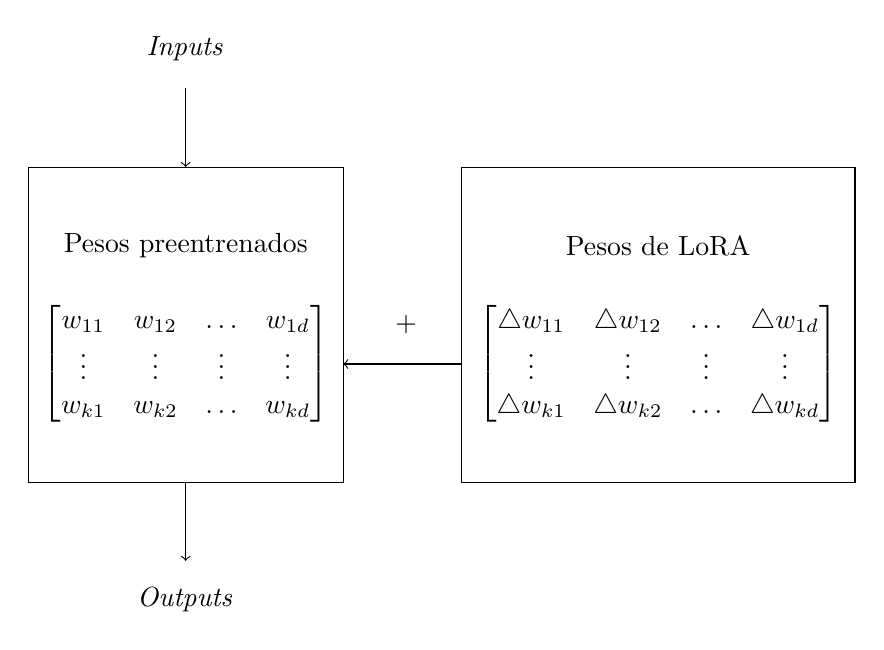
\begin{tikzpicture}

% Modelo preentrenado
\draw (0,0) rectangle (4,4);
\node at (2,3) {Pesos preentrenados};
\node at (2, 1.5) {
\(\begin{bmatrix}
w_{11} & w_{12} & \dots & w_{1d} \\
\vdots & \vdots & \vdots & \vdots \\
w_{k1} & w_{k2} & \dots & w_{kd}
\end{bmatrix}\)
};

% LoRA
\draw (5.5,0) rectangle (10.5,4);
\node at (8,3) {Pesos de LoRA};
\node at (8, 1.5) {
\(\begin{bmatrix}
\bigtriangleup  w_{11} & \bigtriangleup  w_{12} & \dots & \bigtriangleup w_{1d} \\
\vdots & \vdots & \vdots & \vdots \\
\bigtriangleup w_{k1} & \bigtriangleup w_{k2} & \dots & \bigtriangleup w_{kd}
\end{bmatrix}\)
};

% Flechas
\node at (2, 5.5) {\textit{Inputs}};
\draw[->] (2,5) -- (2,4);

\node at (2, -1.5) {\textit{Outputs}};
\draw[->] (2, 0) -- (2, -1);

\draw[->] (5.5, 1.5) -- (4, 1.5);
\node at (4.8, 2) {+};
\end{tikzpicture}
\caption{Esquema de las matrices de parámetros de LoRA}
\label{fig:matricesLoRA}
\end{figure}

LoRA se basa en la idea de la descomposición en rangos de las matrices. El rango de una matriz hace referencia al número de columnas linealmente independientes de esta. Una columna es linealmente dependiente si puede ser obtenida como combinación lineal de otras columnas de la matriz. Esto implica que, si existen columnas linealmente dependientes en la matriz, estas se pueden eliminar sin necesidad de perder información, permitiendo así reducir el tamaño de esta.

Así, en lugar de optimizar los pesos de la matriz completa, LoRA utiliza lo que se conoce como \textit{low rank decomposition} (en español, descomposición en rango bajo), de manera que la matriz $\bigtriangleup W$ se representa como el producto de dos matrices:

\begin{equation}
\bigtriangleup W = B \cdot A =
\begin{bmatrix}
b_{11} & \dots & b_{1r} \\
\vdots &  \vdots & \vdots \\
b_{d1} & \dots & b_{dr}
\end{bmatrix}
\cdot
\begin{bmatrix}
a_{11} & \dots & a_{1k} \\
\vdots & \vdots & \vdots \\
a_{r1} & \dots & a_{rk}
\end{bmatrix}
\end{equation}

Aquí, la matriz $B$ tiene dimensiones $d x r$, y la matriz A, $r x k$, donde $d$ es el número de filas de la matriz de pesos original, $k$ es el número de columnas y $r$, es un hiperparámetro (denominado \textit{rank} o rango) que se debe determinar.

Este enfoque proporciona una mayor eficiencia computacional, ya que se está reduciendo el número de elementos en las matrices $A$ y $B$ con respecto a la matriz original. En el entrenamiento, la matriz $A$ se inicializa a partir de una distribución gaussiana, mientras que la matriz $B$ es inicializada a 0. A medida que trascurre el entrenamiento, los pesos se ajustan para adaptar el modelo a la tarea.

En las siguientes secciones presentaremos cuáles son los hiperparámetros que se deben ajustar en un entrenamiento con LoRA.

\subsubsection{Rango}

El primer hiperparámetro que se debe determinar en un entrenamiento con LoRA es el rango (\textit{rank}, $r$). Este representa el rango de la matriz de parámetros original. Su valor exacto es desconocido, por lo que se deberá seleccionar al inicio del entrenamientol. Idealmente, $r$ debe ser lo más pequeño posible, pero aún debe ser suficiente para capturar la información esencial. Se debe tener en cuenta que:

\begin{itemize}
	\item Si $r$ es demasiado pequeño, la matriz se reduce excesivamente, eliminando columnas que no son linealmente dependientes y, por tanto, perdiendo información necesaria.
	\item Si $r$ es demasiado grande, se incluirán parámetros linealmente dependientes, cosa que puede reducir la efectividad computacional.
\end{itemize}

\subsubsection{\textit{Alpha}}

\textit{Alpha} es un parámetro que se utiliza para escalar los pesos entrenados, determinando la importancia que se les debe dar a los pesos aprendidos durante el entrenamiento en el modelo. Se debe tener en cuenta lo siguiente:

\begin{itemize}
	\item Si $\alpha = r$, los nuevos pesos serán integrados con los del modelo original en una proporción de 1:1.
	\item Si $\alpha > r$, se está dando mayor peso a los nuevos parámetros aprendidos. Esto es recomendable únicamente cuando se cuenta con un conjunto de datos de entrenamiento grande y de alta calidad. De lo contrario, al darle más importancia al conocieminto aprendido del nuevo conjunto de datos en lugar de al conociemiento preexistente del modelo, podría resultar en incoherencias.
	\item Si $\alpha < r$, se prioriza el conocimiento preexistente del modelo sobre el nuevo. Esta configuración es aconsejable cuando el conjunto de datos de entrenamiento es pequeño, pues así se garantiza que el modelo conserve más el conociemiento original.
\end{itemize}

\subsubsection{\textit{Dropout}}

El parámetro de \textit{dropout} determina cuál la probabilidad de que uno de los parámetros ajustados en el entrenamiento sea configurado artificialmente a 0 para un lote de entrenamiento específico. Este procedimiento se realiza para evitar problemas de \textit{overfitting}, donde el modelo se ajusta demasiado a los datos de entrenamiento y pierde capacidad de generalización.

%Generalmente, se recomienda utilizar un \textit{dropout} de 0.1 para modelos de 7B y 13B parámetros y reducirlo a 0.05 para modelos de 33B y 65B parámetros. Esto ayuda a mantener un equilibrio adecuado entre regularización y capacidad de aprendizaje del modelo.

\section{Cuantización}

La creciente complejidad de la arquitectura de los modelos de lenguaje grandes hace que se requiera una gran cantidad de recursos computacionales y de memoria para su implementación y utilización. Este requerimiento intensivo de recursos presenta un desafío significativo, especialmente en entornos con limitaciones en el hardware. Por esta razón, en estos contextos es esencial hacer uso de técnicas que permitan la ejecución eficiente de los modelos, sin compromenter sustancialmente su rendimiento. Una de las técnicas más efectivas en este contexto es la cuantización.

La cuantización es un proceso que consiste en convertir los valores de alta  precisión de un modelo, representados normalmente en punto flotante de 32 o 64 bits, a representaciones de menor precisión, generalmente enteros de 8 o 16 bits \cite{choukroun2019low}. Este mapeo de valores continuos de alta precisión a niveles discretos proporciona una gran mejora en términos de computación y memoria, ya que los requisitos de almacenamiento de un modelo de baja precisión son sustancialmente menores que los de uno de alta precisión. Además, también se pueden observar mejoras en cuanto al consumo de energía, los requisitos de ancho de banda de la memoria y la complejidad computacional.

De todas maneras, es importante tener en cuenta que la inferencia con baja precisión de bits puede conllevar a una pérdida de precisión en la tarea. Esta pérdida de precisión puede compensarse mediante varias técnicas.

Una de las técnicas de cuantización más utilizadas es la de precisión mixta \cite{micikevicius2018mixedprecisiontraining}. Esta técnica consiste en utilizar una combinación de representaciones de alta y baja precisión dentro del modelo. Por ejemplo, los pesos del modelo pueden estar almacenados en alta precisión, para asegurar la exactitud, mientras que los cálculos durante el entrenamiento se realizan con menor precisión para aumentar la velocidad y reducir el uso de la memoria. Posteriormente, los gradientes calculados en baja precisión se utilizan para actualizar los pesos originales.

Otra técnia ampliamente utilizada es la de cuantización post entrenamiento \cite{xiao2024smoothquantaccurateefficientposttraining}. Esta técnica se aplica después de que los modelos hayan sido completament entrenados utilizando representaciones de alta precisión (en el caso de los modelos de lenguaje grandes preentrenados, después del preentrenamiento). El bojetivo principal es reducir el tamaño del modelo y los requisitos de cálculo para permitir una implementación más eficiente en cuanto a memoria y computación, sin tener que reentrenar el modelo desde cero. De esta manera, los pesos y, a veces, las activaciones del modelo son convertidos a representaciones de menor precisión, generalmente de 8 bits.

\section{Medidas de evaluación} \label{metricas}

La correcta evaluación de los modelos de lenguaje grandes es crucial para poder medir su desempeño en la realización de tareas. A medida que los modelos se vuelven complejos y capaces de generar texto con mayor coherencia y fluidez, se vuelve indispensable contar con métricas de evaluación que permitan cuantificar su desempeño de manera precisa. Estas métricas no solo pueden ayudarnos a comparar modelos entre sí, sino que también proporcionan información sobre las áreas en las que un modelo puede necesitar mejoras.

En este trabajo, utilizaremos las métricas de BLEU y COMET para la evaluación de los modelos. Ambas se explicarán en detalle a continuación.

\subsection{BLEU}

BLEU (\textit{Bilingual Evaluation Understudy}) \cite{papineni-etal-2002-bleu} es una de las métricas más utilizadas actualmente para la evaluación de modelos en el campo del procesamiento de lenguaje natural. Esta métrica se basa en la premisa de que una frase generada por un modelo es mejor cuanto más se parezca a la frase que habría sido generada por una persona. Para poder calcularla, se necesita el conjunto de frases generadas por el modelo y un conjunto de frases de referencia reales generadas por personas.

El enfoque de BLEU consiste en utilizar una media ponderada de las coincidencias entre la frase generada por el modelo y las frases de referencia reales. Para ello, BLEU calcula la precisión modificada de n-gramas ($p_n$) entre las frase de referencia y la frase generada por el modelo. Para calcular esta precisión modificada, primero se cuentan cuántos n-gramas de la frase generada por el modelo coinciden con los n-gramas de las frases de referencia. Este conteo se realiza utilizando los \textit{clipped n-gram counts}, que limitan la cantidad de veces que un n-grama en particular puede ser contado, basado en su frecuencia en las frases de referencia. A continuación, se suma el total de estos n-gramas limitados para todas las frases candidatas generadas por el modelo.

El cálculo de $p_n$ se formaliza de la siguiente manera:

\begin{equation}
p_n = \frac{\sum_{C \in \{\text{Candidatos}\}} \sum_{\text{n-grama} \in C} Count_{clip}(\text{n-grama})}{\sum_{C \in \{\text{Candidatos}\}} \sum_{\text{n-grama }\in C} Count(\text{n-grama})}
\end{equation}

donde el numerador representa la suma total de los \textit{clipped n-gram counts} para todos los candidatos y el denominador es el conteo total de n-gramas en todas las frases candidatas.

BLEU incorpora también un factor de penalización por brevedad (\textit{brevity penalty}), para evitar premiar las frases generadas que sean mucho más cortas que la frase de referencia. Este factor de penalización por brevedad se define como:

\begin{equation}
BP = 
\begin{cases}
	1 & \text{si } c > r \\
	e^{(1-r/c)} & \text{si } c \le r
\end{cases}
\end{equation}

donde $c$ es la longitud de la frase candidatas generadas por el m odelo y $r$ es la longitud de la frase de referencia.

Finalmente, el valor de BLEU se obtiene combinando estas precisiones de n-gramas modificadas a través de diferentes valores de n:

\begin{equation}
BLEU = BP + exp(\sum_{n = 1}^N w_n log p_n)
\end{equation}

donde generalmente se utilizan los valores de $N = 4$ y $w_n = \frac{1}{N}$.

AÑADIR LIMITACIONES

\subsection{COMET}

COMET (\textit{Crosslingual Optimized Metric for Evaluation of Translation}) \cite{rei2020cometneuralframeworkmt} es una métrica avanzada utilizada para evaluar la calidad de las traducciones generadas por modelos de lenguaje en el campo de la traducción automática. A diferencia de BLEU, que se basa en coincidencias léxicas de n-gramas, COMET utiliza modelos de aprendizaje profundo para capturar de manera más efectiva la calidad de las traducciones.

COMET se presenta en dos tipos de arquitecturas: el \textit{estimator model} y \textit{translation ranking model}. La diferencia entre ambas es el objetivo de entrenamiento, ya que el \textit{estimator model} está diseñado para predecir directamente un \textit{score} de calidad para una traducción dada, mientras que el \textit{translation ranking model} se entrena para minimizar la distancia entre una traducción generada por el modelo y su correspondiente frase de referencia y frase original en el idioma fuente.

Ambos modelos están formados por dos componentes principales:

\begin{itemize}
	\item \textbf{\textit{Cross-lingual encoder}}: es un modelo pre-entrenado multilingüe, por ejemplo BERT, XLM o XLM-RoBERTa. Estos modelos contienen varias capas de codificación de \textit{transformer} que generan representaciones (\textit{embeddings}) de las secuencias de entrada. En el caso de COMET, estas secuencias serán las frases originales, las frases generadas por el modelo y las frases de referencia. Así, el codificador mapea todas estas a un mismo espacio de características, de manera que es posible hacer comparaciones más precisas.
	\item \textbf{\textit{Pooling layer}}: es una capa de agrupamiento que toma los \textit{embeddings} más importantes generados por las capas del codificador y los combina en una única representación fija $e_{x_j}$. Esta representación se calcula como:

\begin{equation}
e_{x_j} = \mu E_{x_j}^T \alpha
\end{equation}

donde $\mu$ es un parámetro entrenable, $E_{x_j}$ es el vector de \textit{embeddings} para el token $x_j$ y $\alpha$ es un vector que corresponde a los pesos entrenables por capas.

Finalmente, estos \textit{embeddings} son agrupados mediante \textit{average pooling} para obtener una la representación final de cada frase.
\end{itemize}

Las representaciones obtenidas son las que se utilizan posteriormente para calcular el \textit{score} (en el caso del \textit{estimator model}) o el ranking (en el caso del \textit{translation ranking model}) de las frases.

\chapter{Resultados experimentales} \label{cap4}

REESCRIBIR: En este capítulo se presenta el experimento principal de este trabajo, que consiste en el entrenamiento de dos modelos de lenguaje grandes preentrenados: Gemma y Llama-3, enfocados en la tarea específica de generar frases de lenguaje natural a partir de palabras clave en el contexto de los Sistemas de Comunicación Aumentativa y Alternativa. A continuación, se detallan los experimentos realizados, las medidas de evaluación empleadas y los resultados obtenidos.

\section{Conjunto de datos}

Para la realización de los experimentos, se han utilizado dos conjuntos de datos distintos, ambos extraídos del portal de la Universidad de Vigo. Ambos conjuntos contienen frases extraídas de los recursos del Portal Aragonés de la Comunicación Aumentativa y Alternativa, acompañada de la lista de lemas o palabras clave asociadas a cada frase. Estas palabras clave han sido seleccionadas por un grupo de anotadores expertos lingüistas.

El primer conjunto de datos incluye un total de 212 frases, todas ellas en español. El segundo conjunto consta de 260 frases, disponibles tanto en español como en inglés.

A continuación, se presentan algunos ejemplos de frases del primer conjunto de datos para ilustrar su formato:

%\begin{center}
%\begin{tabular}{ | c | }
%\hline
	%El policía puso una multa. | policía, poner, un, multa \\
	%El lobo quiere comerlo. | lobo, querer, comer, lo \\
	%La niña escribe en la arena. | niña, escribir, arena \\
	%Los niños juegan en la piscina. | niño, jugar, piscina \\
	%Los cerditos viven felices. | cerditos, vivir, feliz \\
%\hline
%\end{tabular}
%\end{center}

%\noindent\rule{15cm}{0.4pt}

\begin{displayquote}

El policía puso una multa. | policía, poner, un, multa

El lobo quiere comerlo. | lobo, querer, comer, lo

La niña escribe en la arena. | niña, escribir, arena

Los niños juegan en la piscina. | niño, jugar, piscina

Los cerditos viven felices. | cerditos, vivir, feliz

\end{displayquote}

%\noindent\rule{15cm}{0.4pt}

En cuanto al segundo conjunto de datos, se incluyen ejemplos bilingües:

%\begin{center}
%\begin{tabular}{ | c | }
%\hline
	%Su mamá se enfadó.	su, mamá, se, enfadar | His mother got angry.	his, mother, get, angry \\
	%Pili ha metido un gol.	Pili, haber, meter, un, gol | Pili has scored a goal.	Pili, score, a, goal \\
	%La Luna está en el cielo.	Luna, estar, cielo | The moon is in the sky.	moon, be, sky \\
	%Juan encontró un castillo.	Juan, encontrar, castillo | Juan found a castle.	Juan, find, a, castle \\
	%No lo cambiaré.	no, lo, cambiar | I will not change it.	change, it, not  \\
%\hline
%\end{tabular}
%\end{center}

\begin{displayquote}

Su mamá se enfadó.	su, mamá, se, enfadar | His mother got angry.	his, mother, get, angry

Pili ha metido un gol.	Pili, haber, meter, un, gol | Pili has scored a goal.	Pili, score, a, goal 

La Luna está en el cielo.	Luna, estar, cielo | The moon is in the sky.	moon, be, sky 

Juan encontró un castillo.	Juan, encontrar, castillo | Juan found a castle.	Juan, find, a, castle 

No lo cambiaré.	no, lo, cambiar | I will not change it.	change, it, not  

\end{displayquote}

En el segundo conjunto de datos, se encontraron algunos valores nulos en las listas de palabras clave para ciertas frases en español. Estas frases fueron anotadas manualmente para completar la información faltante.

A partir de estos dos conjuntos, se han creado un conjunto de datos para el entrenamiento en español y otro, en inglés.

\begin{itemize}
	\item \textbf{Conjunto en español}: se ha creado a partir de la unión de las frases en español de los dos conjuntos mencionados. Contiene un total de 340 frases, ya que entre los conjuntos originales algunas se encontraban repetidas.
	\item \textbf {Conjunto en inglés}: se ha creado a partir de las frases en inglés del segundo conjunto de datos, por lo que contiene un total de 260 frases.
\end{itemize}

\subsection{Transformación de los datos}

Tal y como se explicó en la Sección \ref{modelosLenguajeGrandes}, para introducir los datos en el modelo de lenguaje es necesario que estos tengan una estructura de \textit{prompt}, que indique al modelo que esperamos una determinada respuesta de él.

Por esta razón, las frases y sus correspondientes palabras clave han sido transformadas a formato \textit{prompt} para crear los conjuntos de datos. Tanto el conjunto de frases en español como el de frases en inglés contienen una sola columna de tipo texto, que siguen el siguiente formato:

\begin{displayquote}
Lemmas: [lista de palabras clave]

Phrase: [frase generada]
\end{displayquote}

Por ejemplo:

\begin{displayquote}
Lemmas: policía poner un multa

Phrase: El policía puso una multa.
\end{displayquote}

Esta será la manera en que los datos entren al modelo durante el entrenamiento. Para los datos de test, se introducirán con el mismo formato pero sin incluir la frase que generan las palabras clave, pues esta debe ser generada por el modelos:

\begin{displayquote}
Lemmas: policía poner un multa

Phrase:
\end{displayquote}

\subsection{Partición de los datos en entrenamiento, test y validación}

Para evaluar los modelos, se utilizará la técnica de \textit{cross-validation}, que consiste en realizar diferentes particiones de los datos en conjuntos de entrenamiento y test, entrenando y evaluando cada partición por separado. Por esta razón, los datos se han dividido en un conjunto de entrenamiento y test para \textit{cross-validation} y un conjunto de validación.

Los datos de validación no serán utilizados para el entrenamiento del modelo, y se utilizarán para la comparación final de resultados entre los modelos. El conjunto de datos de validación ha sido seleccionado de manera aleatoria entre las frases que no presentaban valores nulos.

La Tabla \ref{tab:frases} muestra la cantidad de datos utilizados para los experimentos en español y en inglés:

\begin{table}[!h]
\caption{Número de frases para validación y entrenamiento de los conjuntos de datos en español y en inglés}
\begin{center}
\begin{tabular}{  c || c  c  }
	\ & Conjunto en español & Conjunto en inglés \\
	\hline
	Entrenamiento-Test & 290 & 220 \\
	Validación & 50 & 40
\end{tabular}
\end{center}
\label{tab:frases}
\end{table}

\section{Experimentos realizados con el conjunto en español}

Los modelos utilizados para los experimentos de este trabajo son los modelos Gemma-7B y Llama3-8B. Ambos modelos están disponibles para su uso libre en el portal de \textit{Hugging Face}.

Para el entrenamiento de los modelos, se ha  aplicado el método de adaptación LoRA, que se describe en detalle en la sección \ref{lora}. Este método requiere la configuración de dos parámetros clave: el rango ($r$) y el parámetro \textit{alpha}. Dado que estos parámetros pueden influir significativamente en el rendimiento del modelo, se han realizado experimentos variando sus valores para identificar la configuración óptmia que proporciona mejores resultados.

Para garantizar una evaluación robusta y fiable de los modelos, se ha utilizado la técnica de \textit{cross-validation} con 10 particiones. Esto implica dividir el conjunto de datos en 10 partes iguales. En cada iteración, 9 partes se utilizan para entrenar el modelo y la parte restante, para probarlo. Las particiones se han realizado de manera que, al final del proceso, todos los datos hayan sido utilizados tanto para entrenamiento como para prueba, asegurando que cada dato aparezce solo una vez en el conjunto de prueba.

Se ha entrenado un modelo independiente para cada una de las 10 particiones. Una vez completado el entrenamiento y realizadas las predicciones de estos 10 modelos, se han combinado las predicciones de todos ellos en un solo conjunto de predicciones para calcular las métricas de rendimiento. Las métricas utilizadas para la evaluación son las métricas BLEU y COMET, ambas descritas en la Sección \ref{metricas}.

\subsection{Primeros experimentos con Gemma y Llama-3}

En los primeros experimentos realizados, se ha comparado el rendimiento de los modelos Gemma-7B y Llama3-8B para evaluar cómo se comportan bajo diferentes configuraciones. El enfoque principal fue explorar el impacto del parámetro de rango en la adaptación LoRA, manteniendo un valor fijo para el parámetro \textit{alpha}. Este enfoque sigue la práctica común de fijar el parámetro \textit{alpha} a dos veces el valor del rango. Los valores de rango explorados han sido 16, 32 y 64.

La Tabla \ref{tab: Gemma y Llama} presenta los resultados obtenidos de BLEU y COMET.

\begin{table}[!h]
\caption{\textit{Scores} de BLEU y COMET para los modelo Gemma-7B y Llama3-8B}
\begin{center}
\begin{tabular}{ c c c c c c }
	\ & \ & Gemma-7B & \ & Llama3-8B & \ \\
	\hline
	\textit{Rank} & \textit{Alpha} & BLEU & COMET & BLEU & COMET \\
	\hline
	\hline
	16 & 32 & 52.44 & 88.92 & 65.59 & 92.82 \\
	\hline
	32 & 64 & 44.44 & 87.44 & 66.13 & 93.37 \\
	\hline
	64 & 128 & 55.21 & 87.82 & 67.62 & 93.23 \\
	

\end{tabular}
\end{center}
\label{tab: Gemma y Llama}
\end{table}

\begin{figure}[h]

\begin{subfigure}{0.5\textwidth}
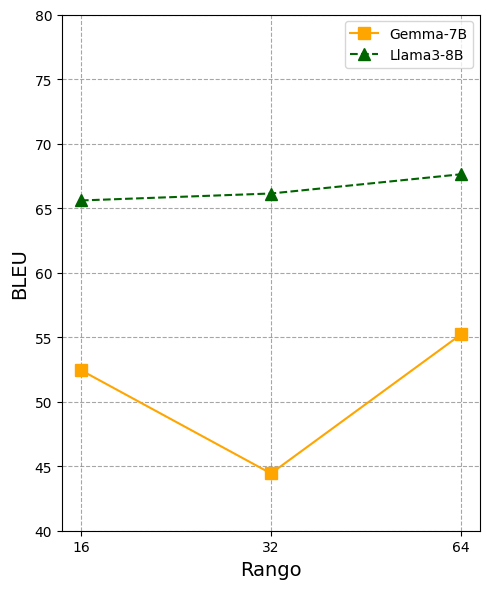
\includegraphics[width=0.9\linewidth, height=9cm]{images/gemma_llama_BLEU} 
\caption{Resultados de BLEU para los modelos Gemma-7B y Llama3-8B}
\label{fig:subim1}
\end{subfigure}
\begin{subfigure}{0.5\textwidth}
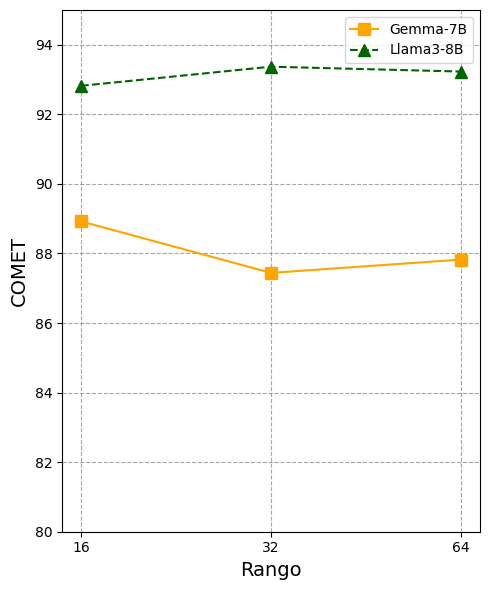
\includegraphics[width=0.9\linewidth, height=9cm]{images/gemma_llama_COMET}
\caption{Resultados de COMET para los modelos Gemma-7B y Llama3-8B}
\label{fig:subim2}
\end{subfigure}

\caption{Resultados obtenidos en las métricas de BLEU y COMET con los modelos Gemma-7B y Llama3-8B tras ser entrenados mediante adaptación con LoRA con los valores de $r$ 16, 32 y 64 y un \textit{alpha} igual a dos veces $r$.}
\label{fig:image2}
\end{figure}

Los resultados muestran que, en todas las configuraciones de rango probadas, el modelo Gemma presenta un rendimiento consistentemente inferior respecto al modelo Llama-3. Esta diferencia de rendimiento sugiere que Llama-3 puede ser más efectivo para las tareas evaluadas.

Dado que Llama-3 ha demostrado ser superior en las pruebas iniciales, se ha decidido que este será el modelo principal a utilizar en los experimentos posteriores. Esta decisión busca maximizar la calidad de los resultados en los experimentos posteriores.

\subsection{Exploración de los valores de \textit{alpha}}

En esta fase de los experimentos, se ha investigado el impacto del parámetro \textit{alpha} en el rendimiento del modelo. El parámetro \textit{alpha} controla el peso relativo que se le asigna a los parámetros de LoRA en comparación con los parámetros del modelo preentrenado. Así, para esta exploración se han realizado experimentos utilizando diferentes valores para el rango $r$ de LoRA: 16, 32, 64 y 128. Para cada valor de $r$, se han probado tres configuraciones distintas de \textit{alpha}:

\begin{enumerate}
	\item \textbf{\textit{alpha} = r/2}: en esta configuración, \textit{alpha} es la mitad del valor del rango. De esta manera, se da más peso a los parámetros del modelo preentrenado y menos a los aprendidos durante el entrenamiento con LoRA.
	\item \textbf{\textit{alpha} = r}: en esta configuración, \textit{alpha} es igual al valor del rango. De esta manera, se da el mismo peso a los parámetros del modelo preentrenado y a los aprendidos durante el entrenamiento con LoRA.
	\item \textbf{\textit{alpha} = 2r}: en esta configuración, \textit{alpha} es el doble del valor del rango. De esta manera, se da más peso a los parámetros aprendidos durante el entrenamiento con LoRA que a los del modelo preentrenado.
\end{enumerate}

Los resultados obtenidos se observan en la Tabla \ref{tab: Llama exploración de alpha}.

\begin{table}[!h]
\caption{\textit{Scores} de BLEU y COMET para el modelo Llama3-8B}
\begin{center}
\begin{tabular}{ c c | c c }
	\hline
	\textit{Rank} & \textit{Alpha} & BLEU & COMET \\
	\hline
	\hline
	16 & 8 & 64.56 & 92.57 \\
	16 & 16 & 65.85 & 92.96 \\
	16 & 32 & 65.59 & 92.82 \\
	\hline
	32 & 16 & 64.55 & 92.95 \\
	32 & 32 & 66.02 & 93.10 \\
	32 & 64 &  66.13 & 93.37 \\
	\hline
	64 & 32 & 68.89 & 93.20\\
	64 & 64 & 67.30 & 93.09\\
	64 & 128 & 67.62 & 93.23\\
	\hline
	128 & 64 & 68.21 & 93.07\\
	128 & 128 & 70.06 & 93.29\\
	128 & 256 & 69.06 & 92.97\\
	

\end{tabular}
\end{center}
\label{tab: Llama exploración de alpha}
\end{table}

\begin{figure}[h]

\begin{subfigure}{0.5\textwidth}
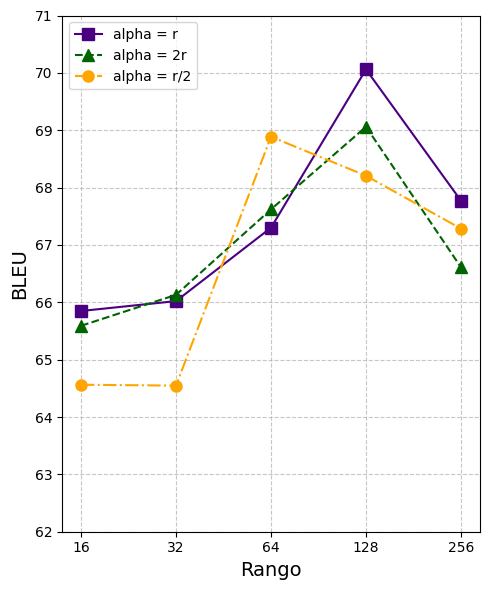
\includegraphics[width=0.9\linewidth, height=9cm]{images/llama_BLEU} 
\caption{Resultados de BLEU para Llama3-8B}
\label{fig:subim1}
\end{subfigure}
\begin{subfigure}{0.5\textwidth}
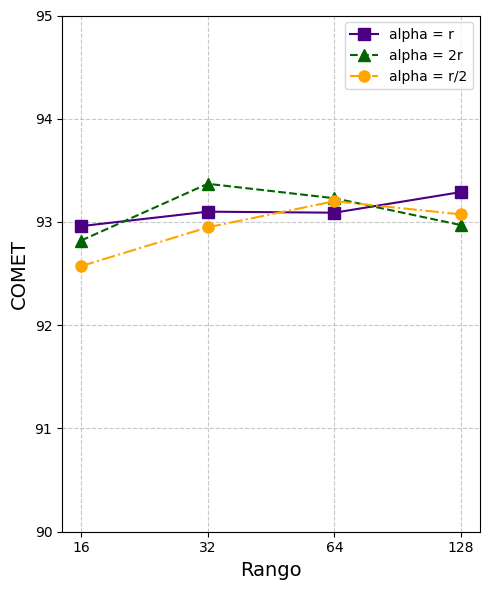
\includegraphics[width=0.9\linewidth, height=9cm]{images/llama_COMET}
\caption{Resultados de COMET para Llama3-8B}
\label{fig:subim2}
\end{subfigure}

\caption{Resultados obtenidos en las métricas de BLEU y COMET conel modelo Llama3-8B tras ser entrenados mediante adaptación con LoRA con los valores de $r$ 16, 32, 64 y 128 y explorando distintos valores de \textit{alpha}.}
\label{fig:graficasLlama}
\end{figure}

En los gráficos de la Figura \ref{fig:graficasLlama} se puede observar visualmente el rendimiento de los diferentes valores de \textit{alpha} en función del parámetro de rango.

En cuanto a la métrica BLEU, los resultados muestran que los experimentos con \textit{alpha} igual a $r/2$ presentan una mayor inestabilidad en comparación con las configuracionies de \textit{alpha} mayores. Los resultados para \textit{alpha} igual a $r$ y \textit{alpha} igual a $2r$ siguen una tendencia más clara y consistente, y en general, muestran un mejor desempeño. Esto sugiere que las configuraciones con valores más altos de \textit{alpha} proporcionan un rendimiento más estable y predecible.

En lo que respecta a la métrica COMET, los resultados muestran que todas las configuraciones de \textit{alpha} se encuentran en un rango de valores de esta métrica similar, sin presentar diferencias notables en su comportamiento.

Para investigar más a fondo, se realizó un experimento adicional con \textit{alpha} igual a $r$ y \textit{alpha} igual a $2r$ utilizando un valor de rango (\textit{r}) de 256. Sin embargo, en este caso, no se observó una tendencia ascendente en el rendimiento.

Así, estos experimentos sugieren que la combinación óptima de parámetros es $r$ igual a 128 con \textit{alpha} igual a $r$.

\subsection{Validación del modelo en español}

Finalmente, se ha llevado a cabo el entrenamiento del modelo de Llama-3 con la mejor combinación de parámetros obtenidos en los experimentos anteriores: $r$ = 128 y \textit{alpha} = $r$. En este caso, el modelo ha sido entrenado utilizando todo el conjunto de datos disponible para el entrenamiento.

Una vez completado el entrenamiento, se ha realizado la validación del modelo utilizando el conjunto de datos reservado específicamente para validación. De esta manera, se ha evaluado el desempeño del modelo en datos que no habían sido vistos por el modelo en ninguna fase de entrenamiento, lo que proporciona una medida de su capacidad de generalización.

Los resultados obtenidos con esta configuración final han sido los siguientes:

\begin{itemize}
	\item BLEU = 62.90
	\item COMET = 89.15
\end{itemize}

Aunque los valores obtenidos para BLEU y COMET son ligeramente inferiores a los resultados alcanzados durante la fase de entrenamiento, estos resultados se encuentran dentro de un rango adecuado de las métricas. La disminución en estas puede deberse a la diferencia entre el conjunto de entrenamiento y el conjunto de validación. De todas maneras, los resultados siguen siendo prometedores y reflejan un buen desempeño del modelo en esta tarea.

\section{Experimentos realizados con el conjunto en inglés}

\section{Comparación con otros modelos}

\begin{table}[!h]
\caption{\textit{Scores} de BLEU y COMET para el modelo Gemma-7B}
\begin{center}
\begin{tabular}{ c c c }
	\ & BLEU & COMET \\
	\hline
	\hline
	Llama-3 & 62.90 & 89.15  \\
	GPT-4 & 66.36 & 92.51\\
	AsTeRICS Grid & 26.89 & 78.36 \\

\end{tabular}
\end{center}
\end{table}

\subsection{Experimentos con personas}

%%%%%%%%%%%%%%%%%%%%%%%%%%%%%%%%%%%%%%%%%%%%%%%%%%%%%%%%%%%%%%%%%%%%%%%%%%%%%%%
%                                 CONCLUSIONS                                 %
%%%%%%%%%%%%%%%%%%%%%%%%%%%%%%%%%%%%%%%%%%%%%%%%%%%%%%%%%%%%%%%%%%%%%%%%%%%%%%%

\chapter{Conclusiones} \label{cap5}

????? ????????????? ????????????? ????????????? ????????????? ????????????? 

\section{Objetivos cumplidos}

\section{}

%%%%%%%%%%%%%%%%%%%%%%%%%%%%%%%%%%%%%%%%%%%%%%%%%%%%%%%%%%%%%%%%%%%%%%%%%%%%%%%
%                                BIBLIOGRAFIA                                 %
%%%%%%%%%%%%%%%%%%%%%%%%%%%%%%%%%%%%%%%%%%%%%%%%%%%%%%%%%%%%%%%%%%%%%%%%%%%%%%%

%%%%%%%%%%%%%%%%%%%%%%%%%%%%%%%%%%%%%%%%%%%%%%%%%%%%%%%%%%%%%%%%%%%%%%%%%%%%%%%
%                                BIBLIOGRAFIA                                 %
%%%%%%%%%%%%%%%%%%%%%%%%%%%%%%%%%%%%%%%%%%%%%%%%%%%%%%%%%%%%%%%%%%%%%%%%%%%%%%%

\bibliographystyle{plain}

\bibliography{plantillatfg}

\cleardoublepage

%%%%%%%%%%%%%%%%%%%%%%%%%%%%%%%%%%%%%%%%%%%%%%%%%%%%%%%%%%%%%%%%%%%%%%%%%%%%%%%
%                           APÈNDIXS  (Si n'hi ha!)                           %
%%%%%%%%%%%%%%%%%%%%%%%%%%%%%%%%%%%%%%%%%%%%%%%%%%%%%%%%%%%%%%%%%%%%%%%%%%%%%%%

\APPENDIX

%%%%%%%%%%%%%%%%%%%%%%%%%%%%%%%%%%%%%%%%%%%%%%%%%%%%%%%%%%%%%%%%%%%%%%%%%%%%%%%
%                         LA CONFIGURACIO DEL SISTEMA                         %
%%%%%%%%%%%%%%%%%%%%%%%%%%%%%%%%%%%%%%%%%%%%%%%%%%%%%%%%%%%%%%%%%%%%%%%%%%%%%%%

\chapter{Configuració del sistema}

????? ????????????? ????????????? ????????????? ????????????? ?????????????

\section{Fase d'inicialització}

????? ????????????? ????????????? ????????????? ????????????? ?????????????

\section{Identificació de dispositius}

????? ????????????? ????????????? ????????????? ????????????? ?????????????

%%%%%%%%%%%%%%%%%%%%%%%%%%%%%%%%%%%%%%%%%%%%%%%%%%%%%%%%%%%%%%%%%%%%%%%%%%%%%%%
%                               ALTRES  APÈNDIXS                              %
%%%%%%%%%%%%%%%%%%%%%%%%%%%%%%%%%%%%%%%%%%%%%%%%%%%%%%%%%%%%%%%%%%%%%%%%%%%%%%%


\chapter{??? ???????????? ????}

????? ????????????? ????????????? ????????????? ????????????? ????????????? 



%%%%%%%%%%%%%%%%%%%%%%%%%%%%%%%%%%%%%%%%%%%%%%%%%%%%%%%%%%%%%%%%%%%%%%%%%%%%%%%
%                              FI DEL DOCUMENT                                %
%%%%%%%%%%%%%%%%%%%%%%%%%%%%%%%%%%%%%%%%%%%%%%%%%%%%%%%%%%%%%%%%%%%%%%%%%%%%%%%

\end{document}
